% Options for packages loaded elsewhere
\PassOptionsToPackage{unicode}{hyperref}
\PassOptionsToPackage{hyphens}{url}
%
\documentclass[
]{book}
\usepackage{amsmath,amssymb}
\usepackage{lmodern}
\usepackage{iftex}
\ifPDFTeX
  \usepackage[T1]{fontenc}
  \usepackage[utf8]{inputenc}
  \usepackage{textcomp} % provide euro and other symbols
\else % if luatex or xetex
  \usepackage{unicode-math}
  \defaultfontfeatures{Scale=MatchLowercase}
  \defaultfontfeatures[\rmfamily]{Ligatures=TeX,Scale=1}
\fi
% Use upquote if available, for straight quotes in verbatim environments
\IfFileExists{upquote.sty}{\usepackage{upquote}}{}
\IfFileExists{microtype.sty}{% use microtype if available
  \usepackage[]{microtype}
  \UseMicrotypeSet[protrusion]{basicmath} % disable protrusion for tt fonts
}{}
\makeatletter
\@ifundefined{KOMAClassName}{% if non-KOMA class
  \IfFileExists{parskip.sty}{%
    \usepackage{parskip}
  }{% else
    \setlength{\parindent}{0pt}
    \setlength{\parskip}{6pt plus 2pt minus 1pt}}
}{% if KOMA class
  \KOMAoptions{parskip=half}}
\makeatother
\usepackage{xcolor}
\IfFileExists{xurl.sty}{\usepackage{xurl}}{} % add URL line breaks if available
\IfFileExists{bookmark.sty}{\usepackage{bookmark}}{\usepackage{hyperref}}
\hypersetup{
  pdftitle={EDV2},
  pdfauthor={Max Brede},
  hidelinks,
  pdfcreator={LaTeX via pandoc}}
\urlstyle{same} % disable monospaced font for URLs
\usepackage{color}
\usepackage{fancyvrb}
\newcommand{\VerbBar}{|}
\newcommand{\VERB}{\Verb[commandchars=\\\{\}]}
\DefineVerbatimEnvironment{Highlighting}{Verbatim}{commandchars=\\\{\}}
% Add ',fontsize=\small' for more characters per line
\usepackage{framed}
\definecolor{shadecolor}{RGB}{248,248,248}
\newenvironment{Shaded}{\begin{snugshade}}{\end{snugshade}}
\newcommand{\AlertTok}[1]{\textcolor[rgb]{0.94,0.16,0.16}{#1}}
\newcommand{\AnnotationTok}[1]{\textcolor[rgb]{0.56,0.35,0.01}{\textbf{\textit{#1}}}}
\newcommand{\AttributeTok}[1]{\textcolor[rgb]{0.77,0.63,0.00}{#1}}
\newcommand{\BaseNTok}[1]{\textcolor[rgb]{0.00,0.00,0.81}{#1}}
\newcommand{\BuiltInTok}[1]{#1}
\newcommand{\CharTok}[1]{\textcolor[rgb]{0.31,0.60,0.02}{#1}}
\newcommand{\CommentTok}[1]{\textcolor[rgb]{0.56,0.35,0.01}{\textit{#1}}}
\newcommand{\CommentVarTok}[1]{\textcolor[rgb]{0.56,0.35,0.01}{\textbf{\textit{#1}}}}
\newcommand{\ConstantTok}[1]{\textcolor[rgb]{0.00,0.00,0.00}{#1}}
\newcommand{\ControlFlowTok}[1]{\textcolor[rgb]{0.13,0.29,0.53}{\textbf{#1}}}
\newcommand{\DataTypeTok}[1]{\textcolor[rgb]{0.13,0.29,0.53}{#1}}
\newcommand{\DecValTok}[1]{\textcolor[rgb]{0.00,0.00,0.81}{#1}}
\newcommand{\DocumentationTok}[1]{\textcolor[rgb]{0.56,0.35,0.01}{\textbf{\textit{#1}}}}
\newcommand{\ErrorTok}[1]{\textcolor[rgb]{0.64,0.00,0.00}{\textbf{#1}}}
\newcommand{\ExtensionTok}[1]{#1}
\newcommand{\FloatTok}[1]{\textcolor[rgb]{0.00,0.00,0.81}{#1}}
\newcommand{\FunctionTok}[1]{\textcolor[rgb]{0.00,0.00,0.00}{#1}}
\newcommand{\ImportTok}[1]{#1}
\newcommand{\InformationTok}[1]{\textcolor[rgb]{0.56,0.35,0.01}{\textbf{\textit{#1}}}}
\newcommand{\KeywordTok}[1]{\textcolor[rgb]{0.13,0.29,0.53}{\textbf{#1}}}
\newcommand{\NormalTok}[1]{#1}
\newcommand{\OperatorTok}[1]{\textcolor[rgb]{0.81,0.36,0.00}{\textbf{#1}}}
\newcommand{\OtherTok}[1]{\textcolor[rgb]{0.56,0.35,0.01}{#1}}
\newcommand{\PreprocessorTok}[1]{\textcolor[rgb]{0.56,0.35,0.01}{\textit{#1}}}
\newcommand{\RegionMarkerTok}[1]{#1}
\newcommand{\SpecialCharTok}[1]{\textcolor[rgb]{0.00,0.00,0.00}{#1}}
\newcommand{\SpecialStringTok}[1]{\textcolor[rgb]{0.31,0.60,0.02}{#1}}
\newcommand{\StringTok}[1]{\textcolor[rgb]{0.31,0.60,0.02}{#1}}
\newcommand{\VariableTok}[1]{\textcolor[rgb]{0.00,0.00,0.00}{#1}}
\newcommand{\VerbatimStringTok}[1]{\textcolor[rgb]{0.31,0.60,0.02}{#1}}
\newcommand{\WarningTok}[1]{\textcolor[rgb]{0.56,0.35,0.01}{\textbf{\textit{#1}}}}
\usepackage{longtable,booktabs,array}
\usepackage{calc} % for calculating minipage widths
% Correct order of tables after \paragraph or \subparagraph
\usepackage{etoolbox}
\makeatletter
\patchcmd\longtable{\par}{\if@noskipsec\mbox{}\fi\par}{}{}
\makeatother
% Allow footnotes in longtable head/foot
\IfFileExists{footnotehyper.sty}{\usepackage{footnotehyper}}{\usepackage{footnote}}
\makesavenoteenv{longtable}
\usepackage{graphicx}
\makeatletter
\def\maxwidth{\ifdim\Gin@nat@width>\linewidth\linewidth\else\Gin@nat@width\fi}
\def\maxheight{\ifdim\Gin@nat@height>\textheight\textheight\else\Gin@nat@height\fi}
\makeatother
% Scale images if necessary, so that they will not overflow the page
% margins by default, and it is still possible to overwrite the defaults
% using explicit options in \includegraphics[width, height, ...]{}
\setkeys{Gin}{width=\maxwidth,height=\maxheight,keepaspectratio}
% Set default figure placement to htbp
\makeatletter
\def\fps@figure{htbp}
\makeatother
\setlength{\emergencystretch}{3em} % prevent overfull lines
\providecommand{\tightlist}{%
  \setlength{\itemsep}{0pt}\setlength{\parskip}{0pt}}
\setcounter{secnumdepth}{5}
\usepackage{booktabs}
\usepackage{tikz}

\newenvironment{cols}[1][]{}{}

\newenvironment{col}[1]{\begin{minipage}{#1}\ignorespaces}{%
\end{minipage}
\ifhmode\unskip\fi
\aftergroup\useignorespacesandallpars}

\def\useignorespacesandallpars#1\ignorespaces\fi{%
#1\fi\ignorespacesandallpars}

\makeatletter
\def\ignorespacesandallpars{%
  \@ifnextchar\par
    {\expandafter\ignorespacesandallpars\@gobble}%
    {}%
}
\makeatother
\usepackage{booktabs}
\usepackage{longtable}
\usepackage{array}
\usepackage{multirow}
\usepackage{wrapfig}
\usepackage{float}
\usepackage{colortbl}
\usepackage{pdflscape}
\usepackage{tabu}
\usepackage{threeparttable}
\usepackage{threeparttablex}
\usepackage[normalem]{ulem}
\usepackage{makecell}
\usepackage{xcolor}
\usepackage{caption}
\usepackage{graphicx}
\usepackage{siunitx}
\usepackage{hhline}
\usepackage{calc}
\usepackage{tabularx}
\usepackage{adjustbox}
\usepackage{hyperref}
\ifLuaTeX
  \usepackage{selnolig}  % disable illegal ligatures
\fi
\usepackage[]{natbib}
\bibliographystyle{apalike}

\title{EDV2}
\author{Max Brede}
\date{2021-05-05}

\begin{document}
\maketitle

{
\setcounter{tocdepth}{1}
\tableofcontents
}
\hypertarget{vorwort}{%
\chapter{Vorwort}\label{vorwort}}

Dieses mit \texttt{bookdown} erstellte Dokument ist das über das Sommersemester 2021 hinweg wachsende Skript zur Übung ``PSY\_B\_12-2: Computerunterstützte Datenanalyse II'' der CAU zu Kiel.

\hypertarget{lehrplan}{%
\chapter{Lehrplan}\label{lehrplan}}

\hypertarget{semesterplan}{%
\section{Semesterplan}\label{semesterplan}}

\hypertarget{uxfcbungsformat}{%
\section{Übungsformat}\label{uxfcbungsformat}}

Die Übung soll zur Hälfte in 45-minütigen Sitzungen im Vorlesungsformat zur Vorstellung der Funktionen und zur anderen Hälfte als 45-minütige praktische Übung stattfinden.
Es wird pro Übungs-Sitzung ein Übungszettel ausgegeben, der mit Hilfe der in der Zugehörigen Vorlesung besprochenen Funktionen bearbeitet werden können soll.
Diese Zettel sollen nach der jeweiligen Vorlesung für die Übungen vorbereitet werden, in denen der Zettel dann besprochen und mögliche Fragen geklärt werden.
Nach den Übungssitzungen haben die Studierenden dann eine Woche Zeit, zusätzliche Hausaufgaben zu bearbeiten.

Eine Ausnahme von diesem Ablauf ist die erste Sitzung, in der organisatorisches und Grundlagen in 90 minütigem Vorlesungsstil besprochen werden sollen. Auch nach dieser Sitzung werden aber Übungszettel und Hausaufgaben ausgegeben.

\hypertarget{lehrziele-fuxfcr-jede-sitzung}{%
\section{Lehrziele für jede Sitzung}\label{lehrziele-fuxfcr-jede-sitzung}}

Die Studierenden können nach dem Absolvieren der Übung\ldots{}

\hypertarget{einheit-1}{%
\subsubsection*{Einheit 1}\label{einheit-1}}
\addcontentsline{toc}{subsubsection}{Einheit 1}

\begin{itemize}
\tightlist
\item
  Gründe für deskriptive Statistik nennen.
\item
  für verschiedene Ausgangssituationen entscheiden, welche Darstellungsform angemessen ist.
\item
  Verfahren zum Umgang mit fehlenden Werten nennen und anwenden.
\item
  Verfahren zum Umgang mit Ausreißern nennen und anwenden.
\end{itemize}

\hypertarget{einheit-2}{%
\subsubsection*{Einheit 2}\label{einheit-2}}
\addcontentsline{toc}{subsubsection}{Einheit 2}

\begin{itemize}
\tightlist
\item
  R \texttt{formula}s lesen und verwenden.
\item
  Korrelationsanalysen in R durchführen und die Ergebnisse interpretieren.
\item
  einfache lineare Regressionen in R durchführen und die Ergebnisse interpretieren.
\end{itemize}

\hypertarget{einheit-3}{%
\subsubsection*{Einheit 3}\label{einheit-3}}
\addcontentsline{toc}{subsubsection}{Einheit 3}

\begin{itemize}
\tightlist
\item
  multiple lineare Regressionen in R durchführen und die Ergebnisse interpretieren.
\end{itemize}

\hypertarget{einheit-4}{%
\subsubsection*{Einheit 4}\label{einheit-4}}
\addcontentsline{toc}{subsubsection}{Einheit 4}

\begin{itemize}
\tightlist
\item
  t-Tests in R durchführen und die Ergebnisse interpretieren.
\item
  einfaktorielle Varianzanalysen in R durchführen und die Ergebnisse interpretieren.
\end{itemize}

\hypertarget{einheit-5}{%
\subsubsection*{Einheit 5}\label{einheit-5}}
\addcontentsline{toc}{subsubsection}{Einheit 5}

\begin{itemize}
\tightlist
\item
  zweifaktorielle Varianzanalysen in R durchführen und die Ergebnisse interpretieren.
\end{itemize}

\hypertarget{einheit-6}{%
\subsubsection*{Einheit 6}\label{einheit-6}}
\addcontentsline{toc}{subsubsection}{Einheit 6}

\begin{itemize}
\tightlist
\item
  beliebige Linearkontraste in R durchführen und die Ergebnisse interpretieren.
\item
  paarweise post-hoc t-Tests in R durchführen und die Ergebnisse interpretieren.
\end{itemize}

\hypertarget{pruxfcfungsleistung}{%
\section{Prüfungsleistung}\label{pruxfcfungsleistung}}

Die Studierenden \textbf{müssen} während des Semesters die nach den Übungssitzungen ausgegebenen Hausaufgaben innerhalb einer Woche sinnvoll bearbeitet abgeben.

Mit maximal einer nicht sinnvoll bearbeiteten Serie werden die Studierenden zur Gruppenarbeit am Ende des Semesters zugelassen.

\hypertarget{deskriptive-statistik-und-data-cleaning}{%
\chapter{Deskriptive Statistik und Data Cleaning}\label{deskriptive-statistik-und-data-cleaning}}

\hypertarget{organisatorisches}{%
\section{Organisatorisches}\label{organisatorisches}}

\hypertarget{semesterplan-1}{%
\subsection{Semesterplan}\label{semesterplan-1}}

\begin{tabular}[t]{llll}
\toprule
Einheit & Vorlesung & Übungswoche & Thema\\
\midrule
1 & 23.04.21 & keine Übung & Deskriptive Statistik\\
 &  &  & Data Cleaning\\
2 & 07.05.21 & KW 19 & Hilfsmittel für die Inferenzstatistik\\
 &  &  & Lineare Regression I\\
3 & 21.05.21 & KW 21 & Lineare Regression II\\
\addlinespace
4 & 04.06.21 & KW 23 & t- Tests\\
 &  &  & einfaktorielle Varianzanalyse\\
5 & 18.06.21 & KW 25 & zweifaktorielle Varianzanalyse\\
6 & 02.07.21 & KW 27 & Kontrasttests\\
\bottomrule
\end{tabular}

\hypertarget{uxfcbungsablauf}{%
\subsection{Übungsablauf}\label{uxfcbungsablauf}}

Es wird alle zwei Wochen eine 45-minütige Vorlesung geben und dazu alternierend online-Übungsstunden in mit je einem Kurs. (Eine Ausnahme ist die erste Woche, in der wir eine Vorlesung haben.)

\hypertarget{uxfcbungsablauf-1}{%
\subsection{Übungsablauf}\label{uxfcbungsablauf-1}}

\begin{center}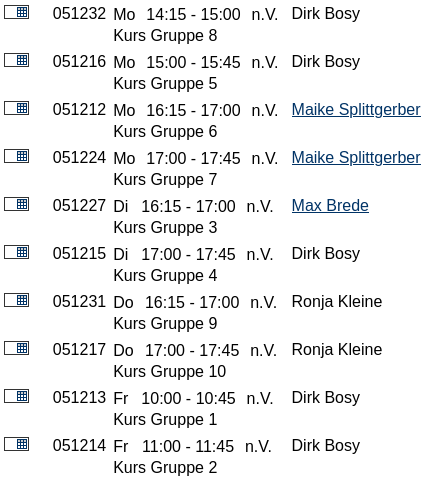
\includegraphics[width=166.666666666667pt]{imgs/univis} \end{center}

\hypertarget{pruxfcfungsleistung-1}{%
\subsection{Prüfungsleistung}\label{pruxfcfungsleistung-1}}

\begin{itemize}
\item
  Gruppenarbeit(4-5 Personen) über 3 Wochen
\item
  Termin für die Klausur entweder vor oder mit Anfang in der Klausurphase.
\end{itemize}

Genauere Informationen gibt es über das Olat.

Als Zulassung für die Gruppenarbeit ist wieder die sinnvolle Bearbeitung von allen bis auf eine Hausaufgabenserien nötig.

\hypertarget{tutorien}{%
\subsection{Tutorien}\label{tutorien}}

Ronja und Katharina geben (online-)Tutorien dieses Semester.

Katharinas Tutorium wird immer dienstags, 14-16 Uhr stattfinden.

Ronjas Tutorium wird immer dienstags, 16-18 Uhr stattfinden.

\hypertarget{deskriptive-statistik}{%
\section{Deskriptive Statistik}\label{deskriptive-statistik}}

\hypertarget{wozu-brauche-ich-das}{%
\subsection{Wozu brauche ich das?}\label{wozu-brauche-ich-das}}

Im Gegensatz zur Inferenzstatistik ist das erklärte Ziel der deskriptiven Statistik, (wie der Name schon sagt) beschreibende Aussagen über die vorliegende Stichprobe zu treffen.

Wir wollen uns also möglichst genau angucken, wie unsere Stichprobe aussieht.

Wozu könnte das gut sein?

\hypertarget{gruxfcnde-fuxfcr-deskriptive-statistik}{%
\subsection{Gründe für deskriptive Statistik}\label{gruxfcnde-fuxfcr-deskriptive-statistik}}

\begin{itemize}
\item
  Indikatoren zur externen Validität(Verteilung von Organismusvariablen, Demografie,\ldots)
\item
  Aussagen über Verteilungseigenschaften

  \begin{itemize}
  \tightlist
  \item
    Schnell zu erfassende Präsentationen von zentraler Tendenz und Streuungen
  \item
    Hinweise auf ungewöhnliche Werte (Ausreißer, fehlende Werte,\ldots)
  \end{itemize}
\item
  Übersicht über Effekte und Zusammenhänge, inklusive solcher, die möglicherweise nicht a-priori erwartet wurden
\end{itemize}

\hypertarget{deskriptive-statistik-1}{%
\subsection{deskriptive Statistik}\label{deskriptive-statistik-1}}

Für einen ganz einfachen, schnellen und umfassenden Überblick über die Daten funktioniert die \texttt{skim}-Funktion aus dem \texttt{skimr}-Paket gut:

\begin{Shaded}
\begin{Highlighting}[]
\NormalTok{skimr}\SpecialCharTok{::}\FunctionTok{skim}\NormalTok{(df)}
\end{Highlighting}
\end{Shaded}

\hypertarget{demografie}{%
\subsection{Demografie}\label{demografie}}

Einfache, schnell zu erfassende Beschreibung der Stichprobe zum Beispiel über eine Tabelle:

\begin{Shaded}
\begin{Highlighting}[]
\NormalTok{df }\SpecialCharTok{\%\textgreater{}\%} 
  \FunctionTok{count}\NormalTok{(sex, smoker, group) }\SpecialCharTok{\%\textgreater{}\%} 
  \FunctionTok{pivot\_wider}\NormalTok{(}\AttributeTok{names\_from =}\NormalTok{ group,}
              \AttributeTok{values\_from =}\NormalTok{ n)}
\end{Highlighting}
\end{Shaded}

\begin{verbatim}
## # A tibble: 4 x 9
##   sex   smoker   g_1   g_2   g_3   g_4   g_6   g_7
##   <chr> <lgl>  <int> <int> <int> <int> <int> <int>
## 1 f     FALSE    373   472   609   384   430   482
## 2 f     TRUE     375   447   634   413   451   474
## 3 m     FALSE    361   441   579   394   442   464
## 4 m     TRUE     397   469   617   358   424   437
##     g_8
##   <int>
## 1   390
## 2   395
## 3   380
## 4   406
\end{verbatim}

Aber vielleicht ein bisschen übersichtlicher in einer Grafik:

\begin{Shaded}
\begin{Highlighting}[]
\NormalTok{df }\SpecialCharTok{\%\textgreater{}\%} 
  \FunctionTok{count}\NormalTok{(sex, smoker, group) }\SpecialCharTok{\%\textgreater{}\%} 
  \FunctionTok{ggplot}\NormalTok{(}\FunctionTok{aes}\NormalTok{(}\AttributeTok{x =}\NormalTok{ group, }\AttributeTok{fill =}\NormalTok{ smoker, }\AttributeTok{y =}\NormalTok{ n)) }\SpecialCharTok{+}
  \FunctionTok{geom\_col}\NormalTok{(}\AttributeTok{position =} \StringTok{\textquotesingle{}dodge\textquotesingle{}}\NormalTok{) }\SpecialCharTok{+}
  \FunctionTok{facet\_wrap}\NormalTok{(}\SpecialCharTok{\textasciitilde{}}\NormalTok{sex) }\SpecialCharTok{+}
  \FunctionTok{labs}\NormalTok{(}\AttributeTok{x =} \StringTok{\textquotesingle{}Group\textquotesingle{}}\NormalTok{,}
       \AttributeTok{y =} \StringTok{\textquotesingle{}Count\textquotesingle{}}\NormalTok{,}
       \AttributeTok{fill =} \StringTok{\textquotesingle{}Smoker\textquotesingle{}}\NormalTok{)}
\end{Highlighting}
\end{Shaded}

\begin{center}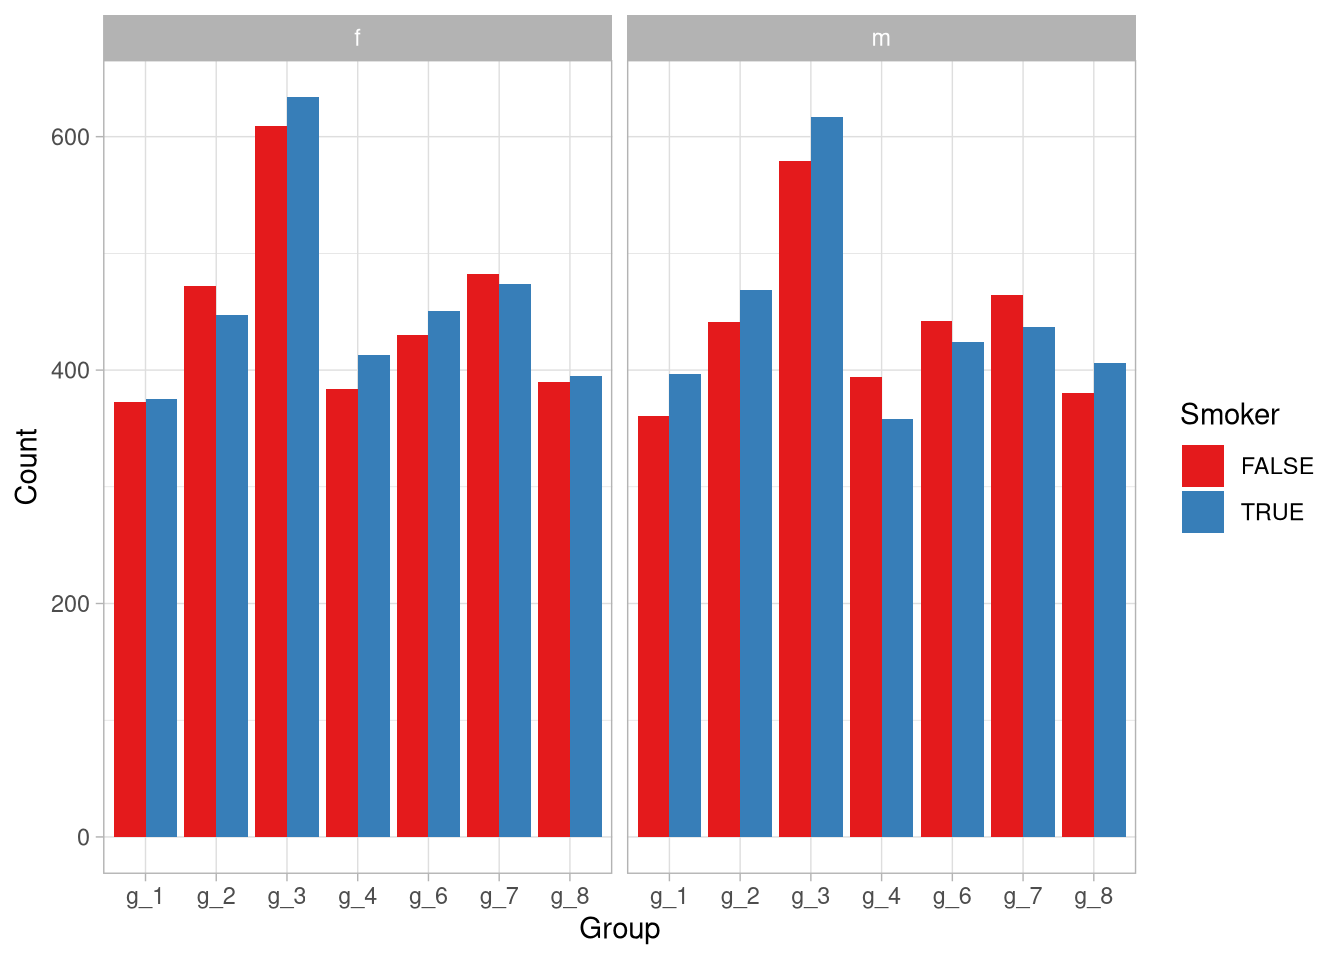
\includegraphics[width=300pt]{EDV2_SS21_files/figure-latex/unnamed-chunk-9-1} \end{center}

Man sieht auf einen Blick, dass Geschlecht und Raucher ungefähr gleich aufgeteilt wurden, die Gruppen aber wesentlich unterschiedliche Größen aufweisen!

\hypertarget{aussagen-uxfcber-verteilungseigenschaften}{%
\subsection{Aussagen über Verteilungseigenschaften}\label{aussagen-uxfcber-verteilungseigenschaften}}

In der \texttt{skim}-Ausgabe haben wir ja schon sehen können, dass keine fehlenden Werte vorliegen (\texttt{n\_missing} war 0).

Wir könnten uns aber noch die Frage stellen, ob Extremwerte in den Gruppen auftauchen, außerdem wollen wir möglichst übersichtlich unsere Verteilungseigenschaften präsentieren.

Das hilft uns zum Einen, um einen besseren Überblick über die Daten zu erhalten, die wir auswerten wollen, zum Anderen hilft es bei einem späteren Bereicht der Leserin, unsere Statistik einzuschätzen.
Dazu können wir uns entweder eine Tabelle mit den Verteilungsparametern der numerischen Variablen ausgeben lassen:

\begin{Shaded}
\begin{Highlighting}[]
\NormalTok{df }\SpecialCharTok{\%\textgreater{}\%} 
  \FunctionTok{pivot\_longer}\NormalTok{(}\FunctionTok{where}\NormalTok{(is.numeric),}
               \AttributeTok{names\_to =} \StringTok{\textquotesingle{}variable\textquotesingle{}}\NormalTok{) }\SpecialCharTok{\%\textgreater{}\%} 
  \FunctionTok{group\_by}\NormalTok{(variable) }\SpecialCharTok{\%\textgreater{}\%} 
  \FunctionTok{summarise}\NormalTok{(}\FunctionTok{across}\NormalTok{(}
\NormalTok{    value,}
    \FunctionTok{list}\NormalTok{(}
      \AttributeTok{mean =} \SpecialCharTok{\textasciitilde{}} \FunctionTok{mean}\NormalTok{(.),}
      \AttributeTok{sd =} \SpecialCharTok{\textasciitilde{}} \FunctionTok{sd}\NormalTok{(.),}
      \AttributeTok{min =} \SpecialCharTok{\textasciitilde{}} \FunctionTok{min}\NormalTok{(.),}
      \AttributeTok{q1 =} \SpecialCharTok{\textasciitilde{}} \FunctionTok{quantile}\NormalTok{(., .}\DecValTok{25}\NormalTok{),}
      \AttributeTok{median =} \SpecialCharTok{\textasciitilde{}} \FunctionTok{median}\NormalTok{(.),}
      \AttributeTok{q3 =} \SpecialCharTok{\textasciitilde{}} \FunctionTok{quantile}\NormalTok{(., .}\DecValTok{75}\NormalTok{),}
      \AttributeTok{max =} \SpecialCharTok{\textasciitilde{}} \FunctionTok{max}\NormalTok{(.)}
\NormalTok{    ),}
    \AttributeTok{.names =} \StringTok{\textquotesingle{}\{.fn\}\textquotesingle{}}
\NormalTok{  )) }\SpecialCharTok{\%\textgreater{}\%} 
  \FunctionTok{mutate}\NormalTok{(}\FunctionTok{across}\NormalTok{(}\FunctionTok{where}\NormalTok{(is.numeric),}
                \SpecialCharTok{\textasciitilde{}}\FunctionTok{round}\NormalTok{(.,}\DecValTok{2}\NormalTok{)))}
\end{Highlighting}
\end{Shaded}

\begin{verbatim}
## # A tibble: 2 x 8
##   variable  mean    sd   min    q1 median    q3   max
##   <chr>    <dbl> <dbl> <dbl> <dbl>  <dbl> <dbl> <dbl>
## 1 age         40    20  17.8  25     32.2  53.6  88.7
## 2 IQ         100    15  69.7  87.3  101.  113.  127.
\end{verbatim}

Oder, wieder ein bisschen übersichtlicher, in einem Diagramm. So könnten wir die ganzen Infos gerade zum Beispiel in einem Boxplot mit eingezeichneten Mittelwerten und Streuungsbalken darstellen:

\begin{Shaded}
\begin{Highlighting}[]
\NormalTok{df }\SpecialCharTok{\%\textgreater{}\%} 
  \FunctionTok{pivot\_longer}\NormalTok{(}\FunctionTok{where}\NormalTok{(is.numeric),}
               \AttributeTok{names\_to =} \StringTok{\textquotesingle{}variable\textquotesingle{}}\NormalTok{) }\SpecialCharTok{\%\textgreater{}\%}  
  \FunctionTok{ggplot}\NormalTok{(}\FunctionTok{aes}\NormalTok{(}\AttributeTok{x =} \StringTok{\textquotesingle{}\textquotesingle{}}\NormalTok{, }\AttributeTok{y =}\NormalTok{ value)) }\SpecialCharTok{+}
  \FunctionTok{geom\_violin}\NormalTok{(}\AttributeTok{fill =} \StringTok{\textquotesingle{}lightgrey\textquotesingle{}}\NormalTok{, }\AttributeTok{color =} \ConstantTok{NA}\NormalTok{) }\SpecialCharTok{+}
  \FunctionTok{geom\_boxplot}\NormalTok{(}\AttributeTok{width =}\NormalTok{ .}\DecValTok{25}\NormalTok{) }\SpecialCharTok{+}
  \FunctionTok{stat\_summary}\NormalTok{(}\AttributeTok{fun =}\NormalTok{ mean, }
               \AttributeTok{fun.min =} \ControlFlowTok{function}\NormalTok{(x)}\FunctionTok{mean}\NormalTok{(x) }\SpecialCharTok{{-}} \FunctionTok{sd}\NormalTok{(x), }
               \AttributeTok{fun.max =} \ControlFlowTok{function}\NormalTok{(x)}\FunctionTok{mean}\NormalTok{(x) }\SpecialCharTok{+} \FunctionTok{sd}\NormalTok{(x),}
               \AttributeTok{color =} \StringTok{\textquotesingle{}red\textquotesingle{}}\NormalTok{) }\SpecialCharTok{+}
  \FunctionTok{facet\_wrap}\NormalTok{(}\SpecialCharTok{\textasciitilde{}}\NormalTok{variable, }\AttributeTok{scales =} \StringTok{\textquotesingle{}free\textquotesingle{}}\NormalTok{) }\SpecialCharTok{+}
  \FunctionTok{labs}\NormalTok{(}\AttributeTok{x =} \StringTok{\textquotesingle{}\textquotesingle{}}\NormalTok{,}
       \AttributeTok{y =} \StringTok{\textquotesingle{}\textquotesingle{}}\NormalTok{)}
\end{Highlighting}
\end{Shaded}

\begin{center}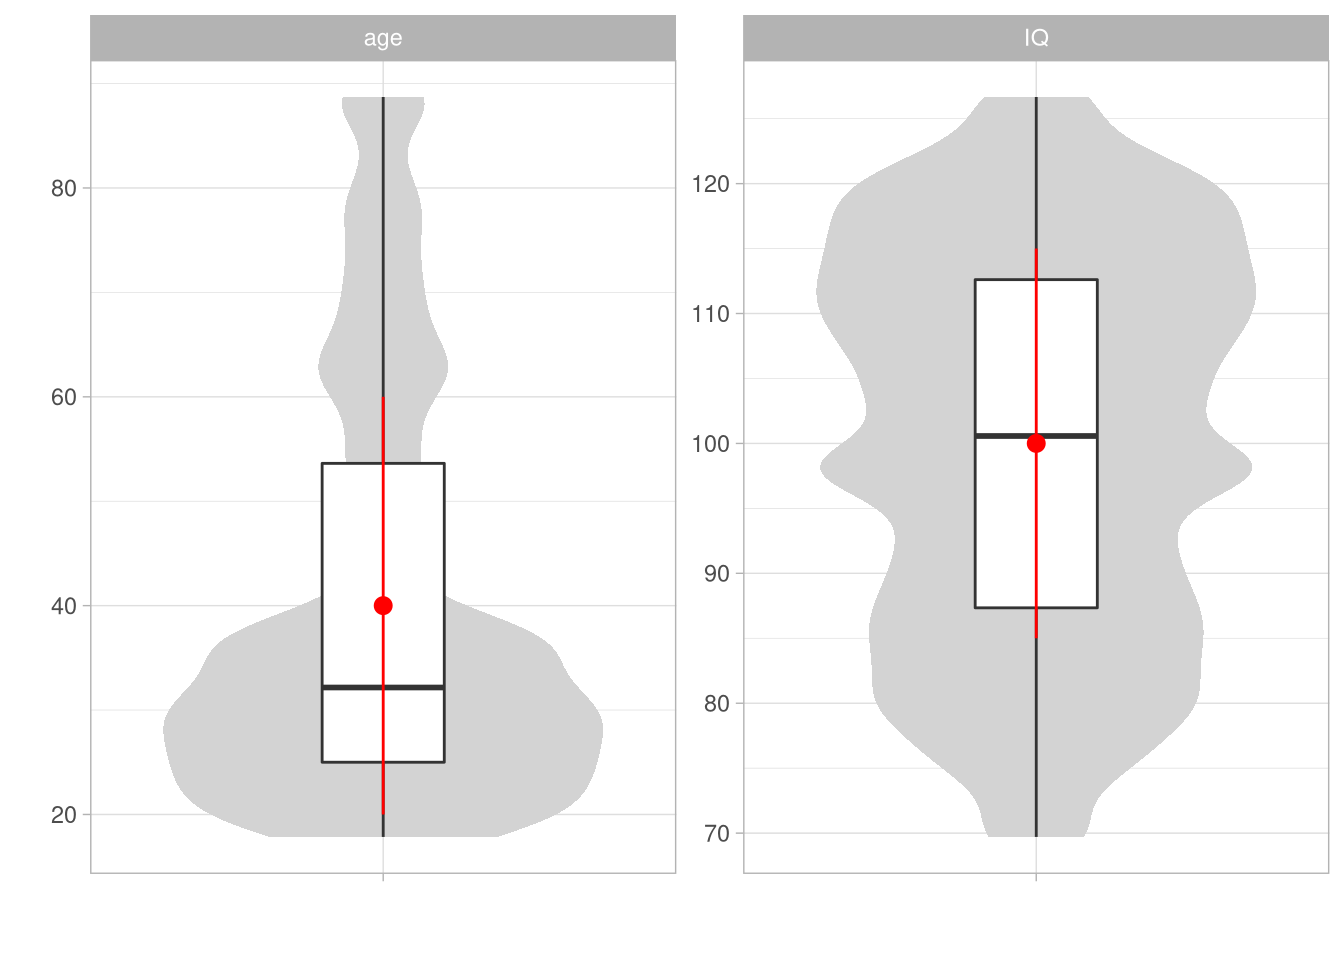
\includegraphics[width=300pt]{EDV2_SS21_files/figure-latex/unnamed-chunk-11-1} \end{center}

Das Alter ist eindeutig schief verteilt, der IQ dafür mehrgipflig.

Nach der von Tukey aufgestellten Regel \citep{tukeyExploratoryDataAnalysis1977} haben wir auch keine Ausreißer (dazu auch später mehr).

\hypertarget{darstellung-von-effekten-und-zusammenhuxe4ngen}{%
\subsection{Darstellung von Effekten und Zusammenhängen}\label{darstellung-von-effekten-und-zusammenhuxe4ngen}}

\hypertarget{unterschiede}{%
\subsubsection{Unterschiede}\label{unterschiede}}

Da wir eine Reihe von Gruppierungsvariablen haben, könnte der erste Impuls sein, sich die Variablen nach diesen Gruppen aufgeteilt darstellen zu lassen, um mögliche Gruppenunterschiede zu verdeutlichen.

Auch hier können wir uns Tabellen erstellen:

\begin{Shaded}
\begin{Highlighting}[]
\NormalTok{df }\SpecialCharTok{\%\textgreater{}\%} 
  \FunctionTok{group\_by}\NormalTok{(smoker, group, sex) }\SpecialCharTok{\%\textgreater{}\%} 
  \FunctionTok{summarise}\NormalTok{(}\FunctionTok{across}\NormalTok{(}\FunctionTok{where}\NormalTok{(is.numeric),}
                   \AttributeTok{.fns =} \FunctionTok{list}\NormalTok{(}\AttributeTok{mean =} \SpecialCharTok{\textasciitilde{}}\FunctionTok{mean}\NormalTok{(.),}
                               \AttributeTok{sd =} \SpecialCharTok{\textasciitilde{}}\FunctionTok{sd}\NormalTok{(.),}
                               \AttributeTok{n =} \SpecialCharTok{\textasciitilde{}}\FunctionTok{n}\NormalTok{()))) }\SpecialCharTok{\%\textgreater{}\%} 
  \FunctionTok{mutate}\NormalTok{(}\FunctionTok{across}\NormalTok{(}\FunctionTok{where}\NormalTok{(is.numeric),}
                \SpecialCharTok{\textasciitilde{}}\FunctionTok{round}\NormalTok{(.,}\DecValTok{2}\NormalTok{)))}
\end{Highlighting}
\end{Shaded}

\begin{verbatim}
## # A tibble: 28 x 9
## # Groups:   smoker, group [14]
##    smoker group sex   IQ_mean IQ_sd  IQ_n age_mean
##    <lgl>  <chr> <chr>   <dbl> <dbl> <dbl>    <dbl>
##  1 FALSE  g_1   f        99.0  13.9   373     31.8
##  2 FALSE  g_1   m        98.4  13.9   361     30.6
##  3 FALSE  g_2   f        98.9  19.3   472     52.0
##  4 FALSE  g_2   m        97.4  19.0   441     53.0
##  5 FALSE  g_3   f       102.   14.0   609     42.5
##  6 FALSE  g_3   m       102.   13.7   579     41.7
##  7 FALSE  g_4   f       101.   13.8   384     40.8
##  8 FALSE  g_4   m        99.3  13.1   394     42.0
##  9 FALSE  g_6   f        99.3  14.6   430     34.8
## 10 FALSE  g_6   m       101.   15.4   442     35.9
##    age_sd age_n
##     <dbl> <dbl>
##  1   17.3   373
##  2   15.3   361
##  3   27.9   472
##  4   27.7   441
##  5   18.2   609
##  6   17.4   579
##  7   19.3   384
##  8   20.3   394
##  9   14.6   430
## 10   14.9   442
## # ... with 18 more rows
\end{verbatim}

Oder Plots erstellen um die möglichen Unterschiede darzustellen:

\begin{Shaded}
\begin{Highlighting}[]
\NormalTok{df }\SpecialCharTok{\%\textgreater{}\%} 
  \FunctionTok{pivot\_longer}\NormalTok{(}\AttributeTok{cols =} \FunctionTok{where}\NormalTok{(is.numeric),}
               \AttributeTok{names\_to =} \StringTok{\textquotesingle{}variable\textquotesingle{}}\NormalTok{) }\SpecialCharTok{\%\textgreater{}\%} 
  \FunctionTok{group\_by}\NormalTok{(variable, smoker, sex, group) }\SpecialCharTok{\%\textgreater{}\%} 
  \FunctionTok{summarise}\NormalTok{(}\AttributeTok{m =} \FunctionTok{mean}\NormalTok{(value),}
            \AttributeTok{sem =} \FunctionTok{sqrt}\NormalTok{(}\FunctionTok{var}\NormalTok{(value)}\SpecialCharTok{/}\FunctionTok{n}\NormalTok{()),}
            \AttributeTok{upper =}\NormalTok{ m }\SpecialCharTok{+}\NormalTok{ sem,}
            \AttributeTok{lower =}\NormalTok{ m }\SpecialCharTok{{-}}\NormalTok{ sem) }\SpecialCharTok{\%\textgreater{}\%} 
  \FunctionTok{ggplot}\NormalTok{(}\FunctionTok{aes}\NormalTok{(}\AttributeTok{x =}\NormalTok{ group,}
             \AttributeTok{y =}\NormalTok{ m,}
             \AttributeTok{fill =}\NormalTok{ smoker)) }\SpecialCharTok{+}
  \FunctionTok{geom\_col}\NormalTok{(}\AttributeTok{position =} \StringTok{\textquotesingle{}dodge\textquotesingle{}}\NormalTok{) }\SpecialCharTok{+}
  \FunctionTok{geom\_errorbar}\NormalTok{(}\FunctionTok{aes}\NormalTok{(}\AttributeTok{ymin =}\NormalTok{ lower,}
                    \AttributeTok{ymax =}\NormalTok{ upper),}
                \AttributeTok{position =} \StringTok{\textquotesingle{}dodge\textquotesingle{}}\NormalTok{)}\SpecialCharTok{+}
  \FunctionTok{facet\_grid}\NormalTok{( variable }\SpecialCharTok{\textasciitilde{}}\NormalTok{ sex , }\AttributeTok{scales =} \StringTok{\textquotesingle{}free\textquotesingle{}}\NormalTok{)}
\end{Highlighting}
\end{Shaded}

\begin{center}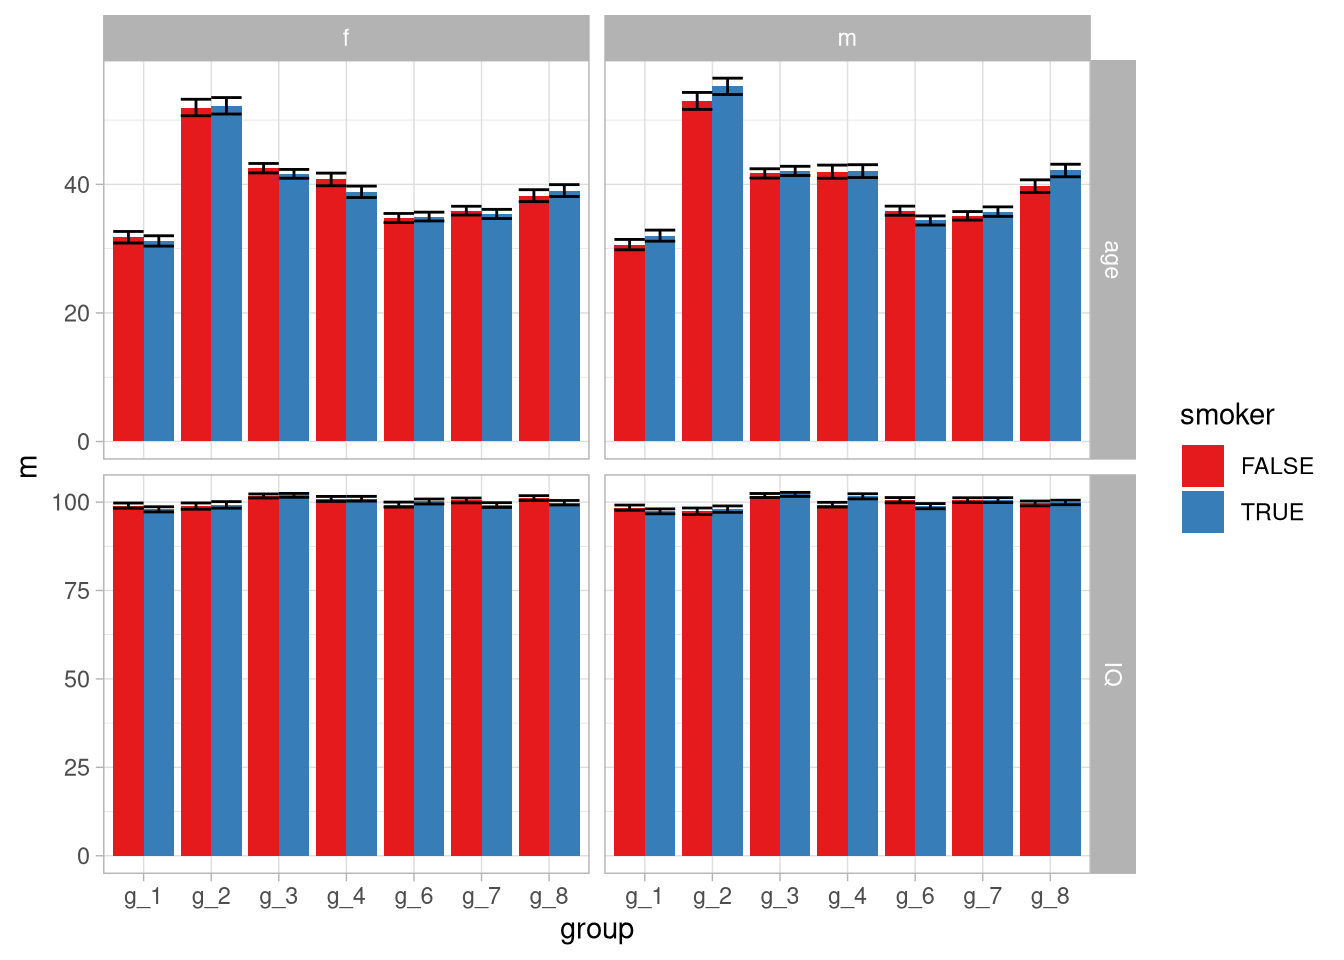
\includegraphics[width=300pt]{EDV2_SS21_files/figure-latex/unnamed-chunk-13-1} \end{center}

Das wird zwar ein bisschen unübersichtlich (wenn man das wirklich sinnvoll betreiben wollen würde sollte man sich Gedanken dazu machen, welche Variablen tatsächlich von Relevanz sind), man könnte aber zu dem Schluss kommen dass die IQs relativ ähnlich sind, die Altersgruppen aber nicht.

\hypertarget{zusammenhuxe4nge}{%
\subsubsection{Zusammenhänge}\label{zusammenhuxe4nge}}

Zuletzt wollen wir noch gucken, ob in den Daten irgendwelche (linearen) Zusammenhänge direkt ersichtlich sind. Dazu können wir zuerst Korrelationen berechnen, zum Beispiel einmal für die gesamte Stichprobe und einmal für die Untergruppen:

\begin{Shaded}
\begin{Highlighting}[]
\FunctionTok{library}\NormalTok{(magrittr)}

\NormalTok{df }\SpecialCharTok{\%$\%} 
  \FunctionTok{cor}\NormalTok{(age,}
\NormalTok{      IQ)}
\end{Highlighting}
\end{Shaded}

\begin{verbatim}
## [1] 0.06659135
\end{verbatim}

\begin{Shaded}
\begin{Highlighting}[]
\NormalTok{df }\SpecialCharTok{\%\textgreater{}\%} 
  \FunctionTok{group\_by}\NormalTok{(group) }\SpecialCharTok{\%\textgreater{}\%} 
  \FunctionTok{summarise}\NormalTok{(}\AttributeTok{r =} \FunctionTok{cor}\NormalTok{(age, IQ))}
\end{Highlighting}
\end{Shaded}

\begin{verbatim}
## # A tibble: 7 x 2
##   group       r
##   <chr>   <dbl>
## 1 g_1   0.0540 
## 2 g_2   0.00747
## 3 g_3   0.110  
## 4 g_4   0.0952 
## 5 g_6   0.111  
## 6 g_7   0.139  
## 7 g_8   0.0636
\end{verbatim}

Hier ist so weit nichts auffällig. Ein letzter zu überprüfender Aspekt sind die nicht-linearen Zusammenhänge, zum Beispiel über angemessene Plots. Dies können wir zum Einen für die Untergruppen überprüfen wollen:

\begin{Shaded}
\begin{Highlighting}[]
\NormalTok{df }\SpecialCharTok{\%\textgreater{}\%} 
  \FunctionTok{ggplot}\NormalTok{(}\FunctionTok{aes}\NormalTok{(}\AttributeTok{x =}\NormalTok{ IQ, }
             \AttributeTok{y =}\NormalTok{ age, }
             \AttributeTok{color =}\NormalTok{ group)) }\SpecialCharTok{+}
  \FunctionTok{geom\_point}\NormalTok{() }\SpecialCharTok{+}
  \FunctionTok{facet\_grid}\NormalTok{(smoker }\SpecialCharTok{\textasciitilde{}}\NormalTok{ sex)}
\end{Highlighting}
\end{Shaded}

\begin{center}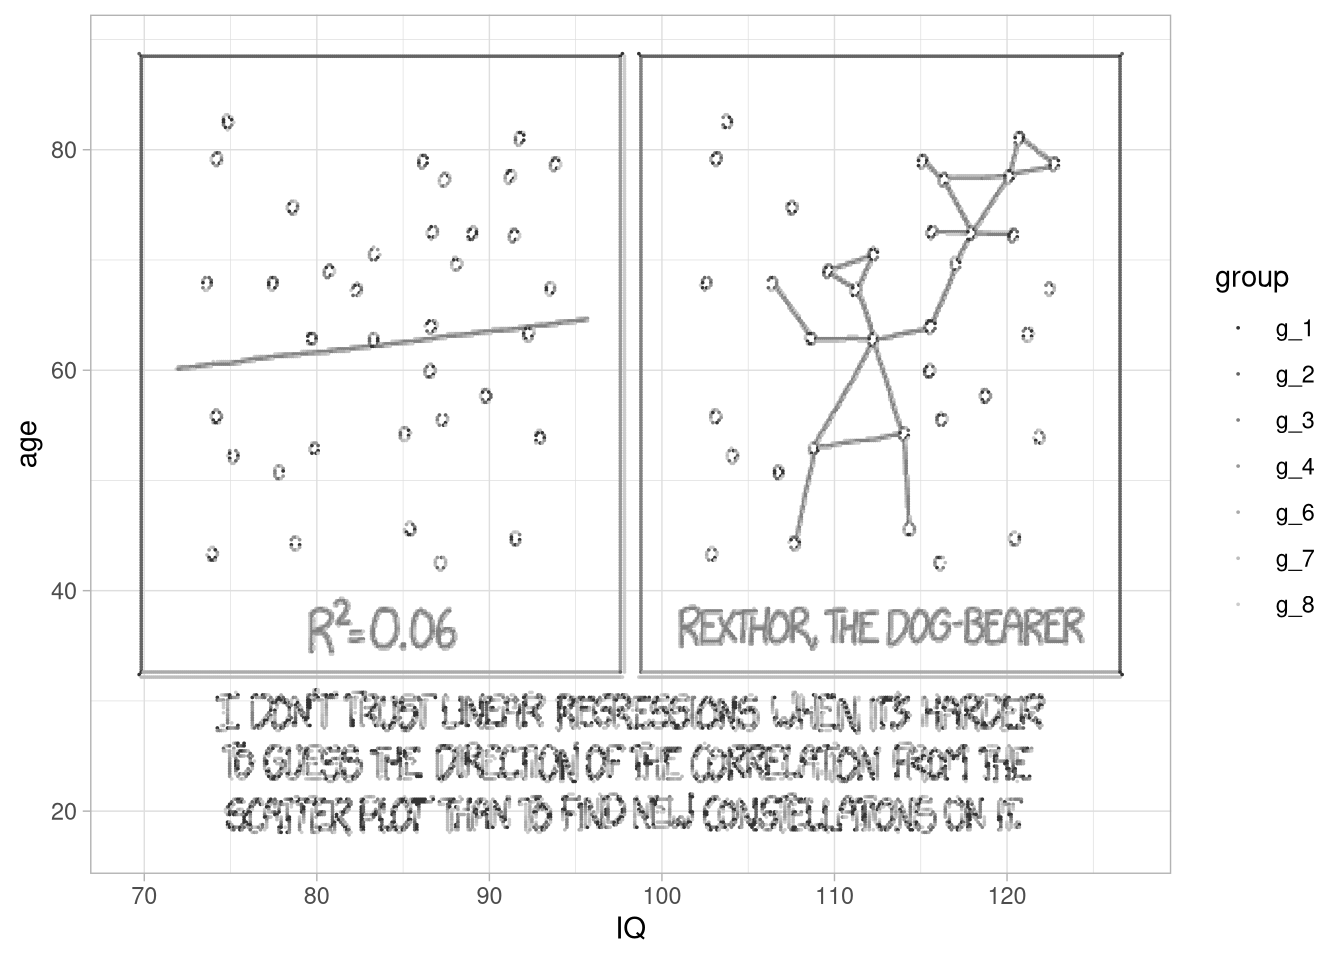
\includegraphics[width=300pt]{EDV2_SS21_files/figure-latex/unnamed-chunk-15-1} \end{center}

Zum Anderen für die gesamte Stichprobe:

\begin{Shaded}
\begin{Highlighting}[]
\NormalTok{df }\SpecialCharTok{\%\textgreater{}\%} 
  \FunctionTok{ggplot}\NormalTok{(}\FunctionTok{aes}\NormalTok{(IQ, age, }\AttributeTok{color =}\NormalTok{ group)) }\SpecialCharTok{+}
  \FunctionTok{geom\_point}\NormalTok{(}\AttributeTok{size =}\NormalTok{ .}\DecValTok{001}\NormalTok{) }\SpecialCharTok{+}
  \FunctionTok{scale\_color\_grey}\NormalTok{()}
\end{Highlighting}
\end{Shaded}

\begin{figure}

{\centering 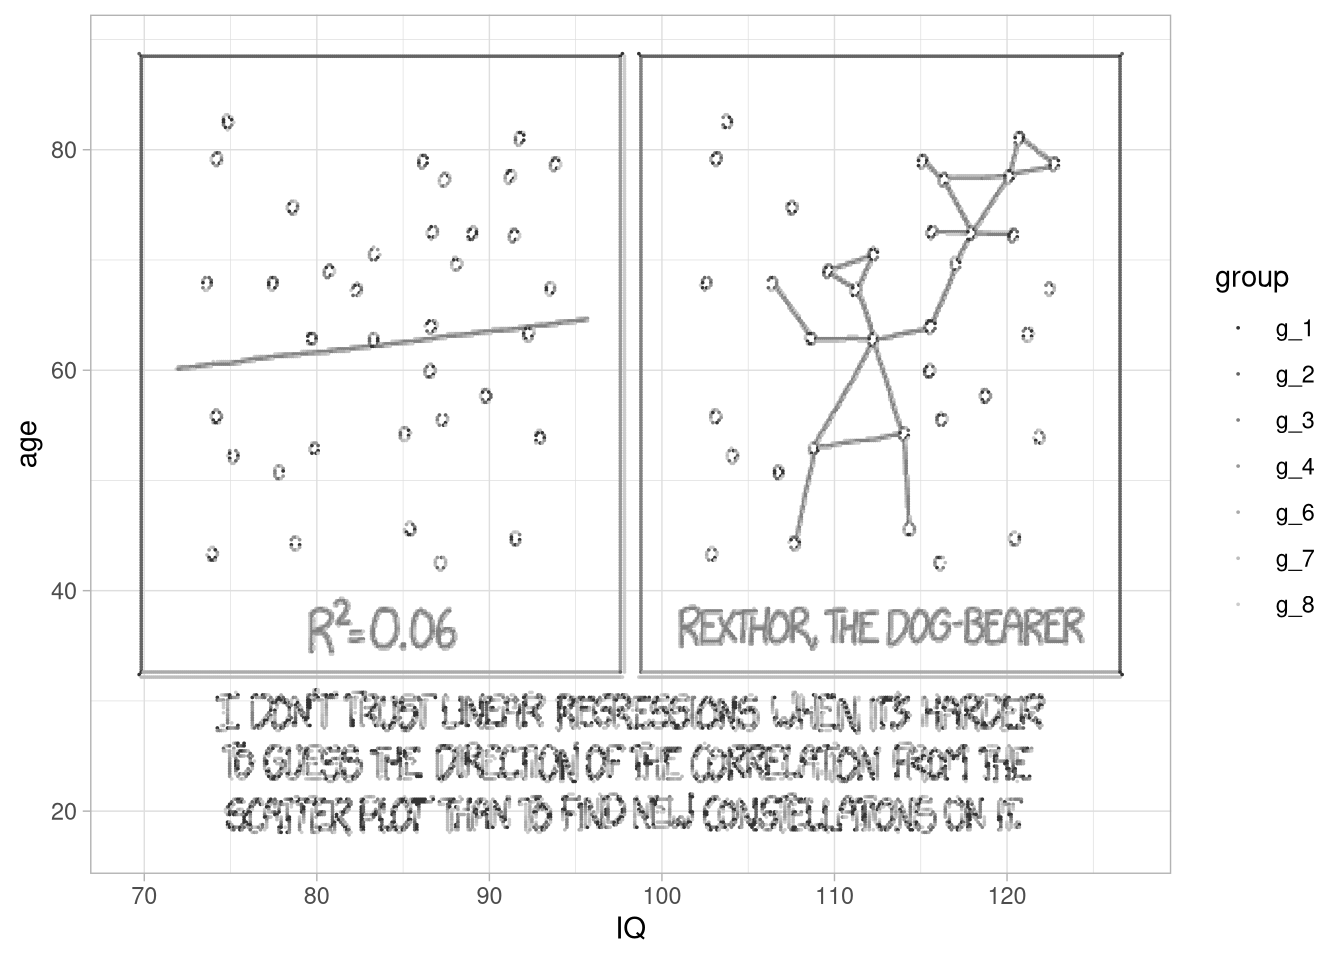
\includegraphics[width=300pt]{EDV2_SS21_files/figure-latex/unnamed-chunk-16-1} 

}

\caption{Original-Comic von [xkcd](https://xkcd.com/1725/)}\label{fig:unnamed-chunk-16}
\end{figure}

\hypertarget{data-cleaning}{%
\section{Data Cleaning}\label{data-cleaning}}

\hypertarget{umgang-mit-fehlenden-werten}{%
\subsection{Umgang mit fehlenden Werten}\label{umgang-mit-fehlenden-werten}}

\texttt{NA}s sind das in R zur Codierung von fehlenden Werten genutzte Datenformat.

Sie können in Vektoren (und damit auch \texttt{tibble}-Spalten) jeden Datenformats auftreten:

\begin{Shaded}
\begin{Highlighting}[]
\FunctionTok{c}\NormalTok{(T,}\ConstantTok{NA}\NormalTok{,F)}
\end{Highlighting}
\end{Shaded}

\begin{verbatim}
## [1]  TRUE    NA FALSE
\end{verbatim}

\begin{Shaded}
\begin{Highlighting}[]
\FunctionTok{c}\NormalTok{(}\DecValTok{1}\NormalTok{,}\ConstantTok{NA}\NormalTok{,}\DecValTok{2}\NormalTok{)}
\end{Highlighting}
\end{Shaded}

\begin{verbatim}
## [1]  1 NA  2
\end{verbatim}

\begin{Shaded}
\begin{Highlighting}[]
\FunctionTok{c}\NormalTok{(}\StringTok{\textquotesingle{}a\textquotesingle{}}\NormalTok{,}\ConstantTok{NA}\NormalTok{,}\StringTok{\textquotesingle{}b\textquotesingle{}}\NormalTok{)}
\end{Highlighting}
\end{Shaded}

\begin{verbatim}
## [1] "a" NA  "b"
\end{verbatim}

Wenn wir versuche mit einem Vektor zu rechnen, der \texttt{NA}s beinhaltet, können wir auf Probleme stoßen:

\begin{Shaded}
\begin{Highlighting}[]
\NormalTok{aVector }\OtherTok{\textless{}{-}} \FunctionTok{c}\NormalTok{(}\ConstantTok{NA}\NormalTok{,}\DecValTok{1}\NormalTok{,}\DecValTok{2}\NormalTok{,}\DecValTok{5}\NormalTok{,}\ConstantTok{NA}\NormalTok{,}\DecValTok{6}\NormalTok{,}\DecValTok{8}\NormalTok{)}
\FunctionTok{length}\NormalTok{(aVector[aVector }\SpecialCharTok{\textgreater{}} \DecValTok{3}\NormalTok{])}
\end{Highlighting}
\end{Shaded}

\begin{verbatim}
## [1] 5
\end{verbatim}

\begin{Shaded}
\begin{Highlighting}[]
\FunctionTok{mean}\NormalTok{(aVector)}
\end{Highlighting}
\end{Shaded}

\begin{verbatim}
## [1] NA
\end{verbatim}

Mit der \texttt{is.na()}-Funktion können wir uns einen logischen Vektor ausgeben lassen, der fehlende Werte codiert. Den können wir dann wie gewohnt benutzen:

\begin{Shaded}
\begin{Highlighting}[]
\FunctionTok{sum}\NormalTok{(}\FunctionTok{is.na}\NormalTok{(aVector))}
\end{Highlighting}
\end{Shaded}

\begin{verbatim}
## [1] 2
\end{verbatim}

\begin{Shaded}
\begin{Highlighting}[]
\FunctionTok{any}\NormalTok{(}\FunctionTok{is.na}\NormalTok{(aVector))}
\end{Highlighting}
\end{Shaded}

\begin{verbatim}
## [1] TRUE
\end{verbatim}

\hypertarget{fehlende-werte-und-einfache-kennwerte}{%
\subsection{fehlende Werte und einfache Kennwerte}\label{fehlende-werte-und-einfache-kennwerte}}

Die meisten Funktionen im \texttt{base\ R} Umfang haben ein \texttt{na.rm}-Argument mit dem wir fehlende Werte von Berechnungen ausschließen können. Das kann an vielen Stellen schon eine sinnvolle Lösung sein, zum Beispiel wenn wir die Infos über die Anzahl fehlender Werte nicht verlieren wollen.

Das könnte dann zum Beispiel so aussehen:

\begin{Shaded}
\begin{Highlighting}[]
\FunctionTok{mean}\NormalTok{(aVector)}
\end{Highlighting}
\end{Shaded}

\begin{verbatim}
## [1] NA
\end{verbatim}

\begin{Shaded}
\begin{Highlighting}[]
\FunctionTok{mean}\NormalTok{(aVector, }\AttributeTok{na.rm =}\NormalTok{ T)}
\end{Highlighting}
\end{Shaded}

\begin{verbatim}
## [1] 4.4
\end{verbatim}

Dieses Argument können wir auch in die gewohnten Pipelines einsetzen.

Als Beispiel nehmen wir diesen kleinen (unrealistisch unvollständigen) Datensatz \texttt{df\_2}:

\begin{Shaded}
\begin{Highlighting}[]
\NormalTok{(df\_2 }\OtherTok{\textless{}{-}} \FunctionTok{read\_csv}\NormalTok{(}\StringTok{\textquotesingle{}data/small\_nas.csv\textquotesingle{}}\NormalTok{))}
\end{Highlighting}
\end{Shaded}

\begin{verbatim}
## # A tibble: 12 x 4
##       VP group    t_1    t_2
##    <dbl> <dbl>  <dbl>  <dbl>
##  1     1     1  3.66  -1.53 
##  2     2     2 NA      3.32 
##  3     3     3  2.23  NA    
##  4     4     4  4.82   4.14 
##  5     5     1  0.142  0.537
##  6     6     2  1.86   5.04 
##  7     7     3 NA      1.46 
##  8     8     4  3.60   3.50 
##  9     9     1  0.353 NA    
## 10    10     2 NA     NA    
## 11    11     3  3.79   2.57 
## 12    12     4  5.37   4.95
\end{verbatim}

Wir könnten jetzt die Pipeline für die Gruppenunterschiede von eben nochmal benutzen, aber um eine Angabe zur Anzahl der fehlenden Werte ergänzen:

\begin{Shaded}
\begin{Highlighting}[]
\NormalTok{df\_2 }\SpecialCharTok{\%\textgreater{}\%} 
  \FunctionTok{group\_by}\NormalTok{(group) }\SpecialCharTok{\%\textgreater{}\%} 
  \FunctionTok{summarise}\NormalTok{(}\FunctionTok{across}\NormalTok{(}\FunctionTok{matches}\NormalTok{(}\StringTok{\textquotesingle{}t\_\textquotesingle{}}\NormalTok{),}
                   \AttributeTok{.fns =} \FunctionTok{list}\NormalTok{(}\AttributeTok{mean =} \SpecialCharTok{\textasciitilde{}}\FunctionTok{mean}\NormalTok{(., }\AttributeTok{na.rm =}\NormalTok{ T),}
                               \AttributeTok{sd =} \SpecialCharTok{\textasciitilde{}}\FunctionTok{sd}\NormalTok{(., }\AttributeTok{na.rm =}\NormalTok{ T),}
                               \AttributeTok{n =} \SpecialCharTok{\textasciitilde{}}\FunctionTok{n}\NormalTok{(),}
                               \AttributeTok{missing =} \SpecialCharTok{\textasciitilde{}}\FunctionTok{sum}\NormalTok{(}\FunctionTok{is.na}\NormalTok{(.))))) }\SpecialCharTok{\%\textgreater{}\%} 
  \FunctionTok{mutate}\NormalTok{(}\FunctionTok{across}\NormalTok{(}\FunctionTok{where}\NormalTok{(is.numeric),}
                \SpecialCharTok{\textasciitilde{}}\FunctionTok{round}\NormalTok{(.,}\DecValTok{2}\NormalTok{)))}
\end{Highlighting}
\end{Shaded}

\begin{verbatim}
## # A tibble: 4 x 9
##   group t_1_mean t_1_sd t_1_n t_1_missing t_2_mean
##   <dbl>    <dbl>  <dbl> <dbl>       <dbl>    <dbl>
## 1     1     1.39   1.97     3           0    -0.5 
## 2     2     1.86  NA        3           2     4.18
## 3     3     3.01   1.1      3           1     2.01
## 4     4     4.6    0.91     3           0     4.2 
##   t_2_sd t_2_n t_2_missing
##    <dbl> <dbl>       <dbl>
## 1   1.46     3           1
## 2   1.22     3           1
## 3   0.79     3           1
## 4   0.73     3           0
\end{verbatim}

\hypertarget{na-bereinigung-von-datensuxe4tzen}{%
\subsection{\texorpdfstring{\texttt{NA}-Bereinigung von Datensätzen}{NA-Bereinigung von Datensätzen}}\label{na-bereinigung-von-datensuxe4tzen}}

Vor statistischen Auswertungen kann es aber einfacher sein, den Datensatz komplett von fehlenden Werten zu bereinigen.

Je nach dem Fall und der Person die man fragt, gibt es verschiedene Vorgehensweisen. Wir gucken uns hier genauer den fallweisen Ausschluss und das ersetzen durch Werte der zentralen Tendenz an.

\emph{Die Entscheidung für das Auffüllen oder das Ausschließen muss von Fall zu Fall gefällt werden!}

Wenn wir zum Beispiel unseren \texttt{df\_2} nochmal angucken, fehlt ein Viertel der Werte.
Hier die Fälle aufzufüllen und so zu tun als würde man mit 133\% der Werte arbeiten, die tatsächlich vorlagen, ist offensichtlich schwierig.
Gleichzeitig wird oft das Argument vorgebracht, dass insbesondere diejenigen Versuchspersonen, die in bestimmten Bedingungen keine Antwort produziert haben ein wichtiger Teil der Stichprobe sind und das Auslassen an sich als Form der Antwort betrachtet werden kann.
Wenn wir diese Versuchspersonen ausschließen, verzerren wir nach diesem Argument also systematisch unsere Stichprobe.

Wichtig ist also vor jeder Bereinigung, Überlegungen darüber anzustellen, was im gegebenen Fall gerade die angemessenste Lösung darstellt.
Bei unserem Datensatz df\_2 sind beide Methoden nicht wirklich gut, der Datensatz ist aber auch extrem.

\hypertarget{fallweiser-ausschluss}{%
\subsubsection{Fallweiser Ausschluss}\label{fallweiser-ausschluss}}

Die radikalste Methode ist der Fallweise Ausschluss, also der Ausschluss aller Eintragungen einer Versuchsperson, die mindestens einen fehlenden Wert vorliegen hat.

Als Erinnerung, hier nochmal unser Datensatz \texttt{df\_2}:

\begin{tabular}[t]{rrrr}
\toprule
VP & group & t\_1 & t\_2\\
\midrule
1 & 1 & 3.6612191 & -1.5337696\\
2 & 2 & NA & 3.3223479\\
3 & 3 & 2.2250924 & NA\\
4 & 4 & 4.8187796 & 4.1387727\\
5 & 1 & 0.1419190 & 0.5373972\\
\addlinespace
6 & 2 & 1.8635821 & 5.0435449\\
7 & 3 & NA & 1.4552116\\
8 & 4 & 3.6001703 & 3.5013055\\
9 & 1 & 0.3530444 & NA\\
10 & 2 & NA & NA\\
\addlinespace
11 & 3 & 3.7877141 & 2.5676322\\
12 & 4 & 5.3706695 & 4.9490249\\
\bottomrule
\end{tabular}

Wir müssten also die Versuchspersonen ausschließen.

Die einfachste Variante dafür ist, den Datensatz ins \texttt{wide}-Format zu überführen (wie er es in unserem Fall schon vorliegt) und mit \texttt{drop\_na} diejenigen Zeilen auszuschließen, die fehlende Werte beinhalten:

\begin{Shaded}
\begin{Highlighting}[]
\NormalTok{df\_2 }\SpecialCharTok{\%\textgreater{}\%} 
  \FunctionTok{drop\_na}\NormalTok{()}
\end{Highlighting}
\end{Shaded}

\begin{verbatim}
## # A tibble: 7 x 4
##      VP group   t_1    t_2
##   <dbl> <dbl> <dbl>  <dbl>
## 1     1     1 3.66  -1.53 
## 2     4     4 4.82   4.14 
## 3     5     1 0.142  0.537
## 4     6     2 1.86   5.04 
## 5     8     4 3.60   3.50 
## 6    11     3 3.79   2.57 
## 7    12     4 5.37   4.95
\end{verbatim}

\hypertarget{ersetzen-fehlender-werte}{%
\subsubsection{Ersetzen fehlender Werte}\label{ersetzen-fehlender-werte}}

Statt radikal alle Fälle auszuschließen, die mindestens einen fehlenden Wert beinhalten, gibt es auch Ansätze, diese aufzufüllen.
Gängige Verfahren hier sind die fehlenden Werte hypothesenunabhängig (also nicht gruppenweise) mit dem (getrimmten) Mittelwert, dem Median oder dem Modus der Gesamtstichprobe aufzufüllen. Die Umsetzung in R sieht dann immer gleich aus, die einzige Änderung findet im Kennwert statt, den man zur Ergänzung wählt.

Hier mal ein Beispiel mit dem getrimmten Mittelwert:

\begin{Shaded}
\begin{Highlighting}[]
\NormalTok{df\_2 }\SpecialCharTok{\%\textgreater{}\%} 
  \FunctionTok{mutate}\NormalTok{(}\FunctionTok{across}\NormalTok{(}\FunctionTok{where}\NormalTok{(is.numeric), }
                \SpecialCharTok{\textasciitilde{}}\FunctionTok{replace\_na}\NormalTok{(., }
                            \FunctionTok{mean}\NormalTok{(.,}
                                 \AttributeTok{na.rm=}\NormalTok{T,}
                                 \AttributeTok{trim =}\NormalTok{ .}\DecValTok{05}\NormalTok{))))}
\end{Highlighting}
\end{Shaded}

\begin{verbatim}
## # A tibble: 12 x 4
##       VP group   t_1    t_2
##    <dbl> <dbl> <dbl>  <dbl>
##  1     1     1 3.66  -1.53 
##  2     2     2 2.87   3.32 
##  3     3     3 2.23   2.66 
##  4     4     4 4.82   4.14 
##  5     5     1 0.142  0.537
##  6     6     2 1.86   5.04 
##  7     7     3 2.87   1.46 
##  8     8     4 3.60   3.50 
##  9     9     1 0.353  2.66 
## 10    10     2 2.87   2.66 
## 11    11     3 3.79   2.57 
## 12    12     4 5.37   4.95
\end{verbatim}

\hypertarget{umgang-mit-ausreiuxdfern}{%
\subsection{Umgang mit Ausreißern}\label{umgang-mit-ausreiuxdfern}}

Ausreißerbereinigung sind ein komplexes Thema, über das viel diskutiert werden kann und auch muss.

Da wir uns hier aber im Rahmen einer praktischen Übung befinden sparen wir uns das und nutzen die weit verbreitete Regel, die \citet{tukeyExploratoryDataAnalysis1977} formuliert hat:

Diejenigen Werte sind als Ausreißer zu betrachten, die außerhalb des Intervals
\[Q_1 - 1.5 \cdot \text{IQR} \leq x \leq Q_3 + 1.5 \cdot \text{IQR}\]
liegen. Diese Regel ist auch der in \texttt{geom\_boxplot} implementierte Standard, den wir ja auch schon zumindest vom Sehen kennen.

Die Frage ist nun, was wir mit eventuell detektierten Ausreißern machen.

Dafür betrachten wir den folgenden Datensatz \texttt{df\_3}:

\begin{Shaded}
\begin{Highlighting}[]
\NormalTok{df\_3 }\SpecialCharTok{\%\textgreater{}\%} 
  \FunctionTok{pivot\_longer}\NormalTok{(}\AttributeTok{cols =} \FunctionTok{everything}\NormalTok{()) }\SpecialCharTok{\%\textgreater{}\%} 
  \FunctionTok{ggplot}\NormalTok{(}\FunctionTok{aes}\NormalTok{(}\AttributeTok{y =}\NormalTok{ value, }\AttributeTok{x =} \StringTok{\textquotesingle{}\textquotesingle{}}\NormalTok{)) }\SpecialCharTok{+}
  \FunctionTok{geom\_boxplot}\NormalTok{() }\SpecialCharTok{+}
  \FunctionTok{geom\_dotplot}\NormalTok{(}\AttributeTok{binaxis =} \StringTok{\textquotesingle{}y\textquotesingle{}}\NormalTok{,}
               \AttributeTok{stackdir =} \StringTok{\textquotesingle{}center\textquotesingle{}}\NormalTok{,}
               \AttributeTok{alpha =}\NormalTok{ .}\DecValTok{5}\NormalTok{,}
               \AttributeTok{fill =} \StringTok{\textquotesingle{}red\textquotesingle{}}\NormalTok{,}
               \AttributeTok{dotsize =}\NormalTok{ .}\DecValTok{5}\NormalTok{) }\SpecialCharTok{+}
  \FunctionTok{facet\_wrap}\NormalTok{(}\SpecialCharTok{\textasciitilde{}}\NormalTok{name,}\AttributeTok{scales =} \StringTok{\textquotesingle{}free\_y\textquotesingle{}}\NormalTok{)}
\end{Highlighting}
\end{Shaded}

\begin{center}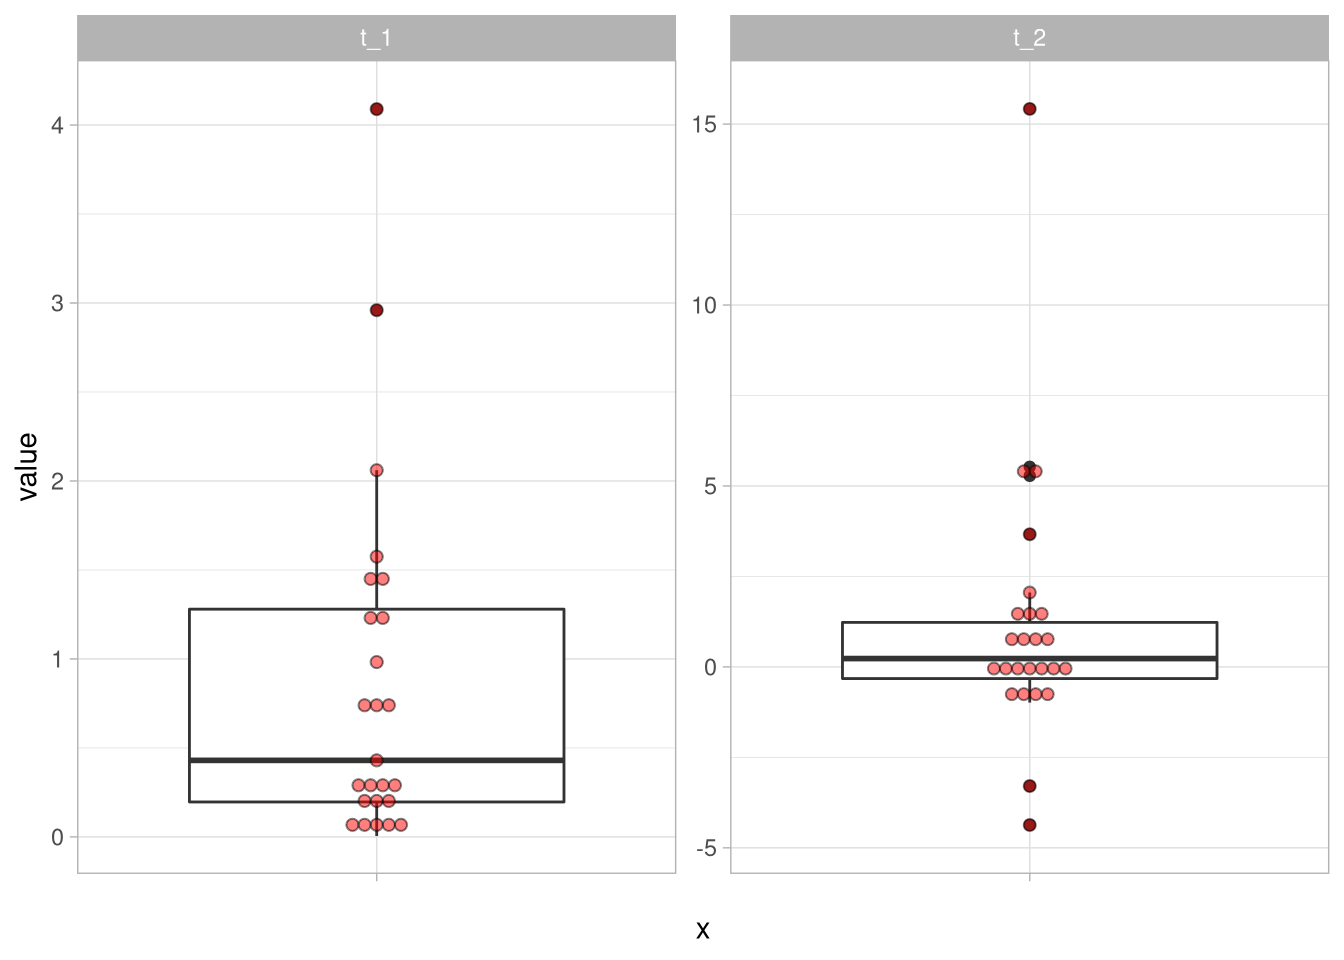
\includegraphics[width=300pt]{EDV2_SS21_files/figure-latex/eval-1} \end{center}

Auch hier können wir wieder zum radikalen Ausschluss greifen und den Datensatz einfach danach filtern, dass unsere Variablen zwischen den ``Tukey Fences'' liegen:

\begin{Shaded}
\begin{Highlighting}[]
\NormalTok{df\_3 }\SpecialCharTok{\%\textgreater{}\%} 
  \FunctionTok{filter}\NormalTok{(}\FunctionTok{between}\NormalTok{(t\_1, }
                 \FunctionTok{quantile}\NormalTok{(t\_1,.}\DecValTok{25}\NormalTok{) }\SpecialCharTok{{-}} \FloatTok{1.5} \SpecialCharTok{*} \FunctionTok{IQR}\NormalTok{(t\_1),}
                 \FunctionTok{quantile}\NormalTok{(t\_1,.}\DecValTok{75}\NormalTok{) }\SpecialCharTok{+} \FloatTok{1.5} \SpecialCharTok{*} \FunctionTok{IQR}\NormalTok{(t\_1)) }\SpecialCharTok{\&}
           \FunctionTok{between}\NormalTok{(t\_2, }
                 \FunctionTok{quantile}\NormalTok{(t\_2,.}\DecValTok{25}\NormalTok{) }\SpecialCharTok{{-}} \FloatTok{1.5} \SpecialCharTok{*} \FunctionTok{IQR}\NormalTok{(t\_2),}
                 \FunctionTok{quantile}\NormalTok{(t\_2,.}\DecValTok{75}\NormalTok{) }\SpecialCharTok{+} \FloatTok{1.5} \SpecialCharTok{*} \FunctionTok{IQR}\NormalTok{(t\_2))) }\SpecialCharTok{\%\textgreater{}\%} 
  \FunctionTok{pivot\_longer}\NormalTok{(}\AttributeTok{cols =} \FunctionTok{everything}\NormalTok{()) }\SpecialCharTok{\%\textgreater{}\%} 
  \FunctionTok{ggplot}\NormalTok{(}\FunctionTok{aes}\NormalTok{(}\AttributeTok{y =}\NormalTok{ value, }\AttributeTok{x =} \StringTok{\textquotesingle{}\textquotesingle{}}\NormalTok{)) }\SpecialCharTok{+}
  \FunctionTok{geom\_boxplot}\NormalTok{() }\SpecialCharTok{+}
  \FunctionTok{geom\_dotplot}\NormalTok{(}\AttributeTok{binaxis =} \StringTok{\textquotesingle{}y\textquotesingle{}}\NormalTok{,}
               \AttributeTok{stackdir =} \StringTok{\textquotesingle{}center\textquotesingle{}}\NormalTok{,}
               \AttributeTok{alpha =}\NormalTok{ .}\DecValTok{5}\NormalTok{,}
               \AttributeTok{fill =} \StringTok{\textquotesingle{}red\textquotesingle{}}\NormalTok{,}
               \AttributeTok{dotsize =}\NormalTok{ .}\DecValTok{5}\NormalTok{) }\SpecialCharTok{+}
  \FunctionTok{facet\_wrap}\NormalTok{(}\SpecialCharTok{\textasciitilde{}}\NormalTok{name,}\AttributeTok{scales =} \StringTok{\textquotesingle{}free\_y\textquotesingle{}}\NormalTok{)}
\end{Highlighting}
\end{Shaded}

\begin{center}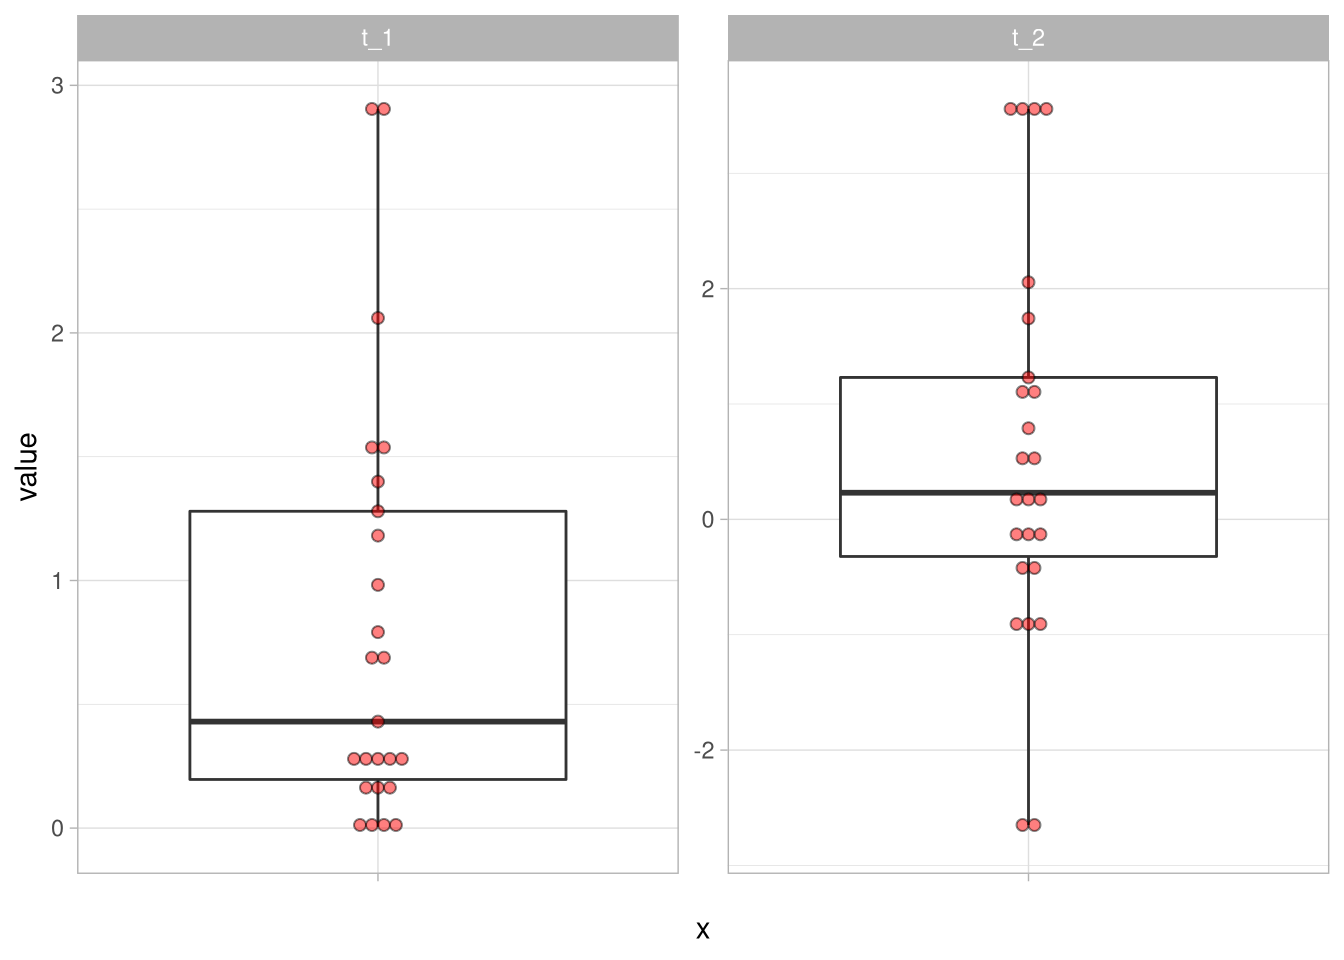
\includegraphics[width=300pt]{EDV2_SS21_files/figure-latex/unnamed-chunk-27-1} \end{center}

Oder wir `windsorieren' unsere Ausreißer, indem wir sie durch den Wert der jeweiligen Grenze ersetzen.
Wir sagen also, dass diejenigen Werte, die außerhalb der Fences liegen auf den Wert der jeweiligen Grenze gesetzt werden sollen:

\begin{Shaded}
\begin{Highlighting}[]
\NormalTok{df\_3 }\SpecialCharTok{\%\textgreater{}\%} 
  \FunctionTok{mutate}\NormalTok{(}\FunctionTok{across}\NormalTok{(}\FunctionTok{everything}\NormalTok{(),}
                \SpecialCharTok{\textasciitilde{}}\FunctionTok{ifelse}\NormalTok{(. }\SpecialCharTok{\textgreater{}}  \FunctionTok{quantile}\NormalTok{(.,.}\DecValTok{75}\NormalTok{) }\SpecialCharTok{+} \FloatTok{1.5} \SpecialCharTok{*} \FunctionTok{IQR}\NormalTok{(.),}
                        \FunctionTok{quantile}\NormalTok{(.,.}\DecValTok{75}\NormalTok{) }\SpecialCharTok{+} \FloatTok{1.5} \SpecialCharTok{*} \FunctionTok{IQR}\NormalTok{(.),}
\NormalTok{                        .)),}
         \FunctionTok{across}\NormalTok{(}\FunctionTok{everything}\NormalTok{(),}
                \SpecialCharTok{\textasciitilde{}}\FunctionTok{ifelse}\NormalTok{(. }\SpecialCharTok{\textless{}}  \FunctionTok{quantile}\NormalTok{(.,.}\DecValTok{25}\NormalTok{) }\SpecialCharTok{{-}} \FloatTok{1.5} \SpecialCharTok{*} \FunctionTok{IQR}\NormalTok{(.),}
                        \FunctionTok{quantile}\NormalTok{(.,.}\DecValTok{25}\NormalTok{) }\SpecialCharTok{{-}} \FloatTok{1.5} \SpecialCharTok{*} \FunctionTok{IQR}\NormalTok{(.),}
\NormalTok{                        .))) }\SpecialCharTok{\%\textgreater{}\%} 
\FunctionTok{pivot\_longer}\NormalTok{(}\AttributeTok{cols =} \FunctionTok{everything}\NormalTok{()) }\SpecialCharTok{\%\textgreater{}\%} 
  \FunctionTok{ggplot}\NormalTok{(}\FunctionTok{aes}\NormalTok{(}\AttributeTok{y =}\NormalTok{ value, }\AttributeTok{x =} \StringTok{\textquotesingle{}\textquotesingle{}}\NormalTok{)) }\SpecialCharTok{+}
  \FunctionTok{geom\_boxplot}\NormalTok{() }\SpecialCharTok{+}
  \FunctionTok{geom\_dotplot}\NormalTok{(}\AttributeTok{binaxis =} \StringTok{\textquotesingle{}y\textquotesingle{}}\NormalTok{,}
               \AttributeTok{stackdir =} \StringTok{\textquotesingle{}center\textquotesingle{}}\NormalTok{,}
               \AttributeTok{alpha =}\NormalTok{ .}\DecValTok{5}\NormalTok{,}
               \AttributeTok{fill =} \StringTok{\textquotesingle{}red\textquotesingle{}}\NormalTok{,}
               \AttributeTok{dotsize =}\NormalTok{ .}\DecValTok{5}\NormalTok{) }\SpecialCharTok{+}
  \FunctionTok{facet\_wrap}\NormalTok{(}\SpecialCharTok{\textasciitilde{}}\NormalTok{name,}\AttributeTok{scales =} \StringTok{\textquotesingle{}free\_y\textquotesingle{}}\NormalTok{)}
\end{Highlighting}
\end{Shaded}

\begin{center}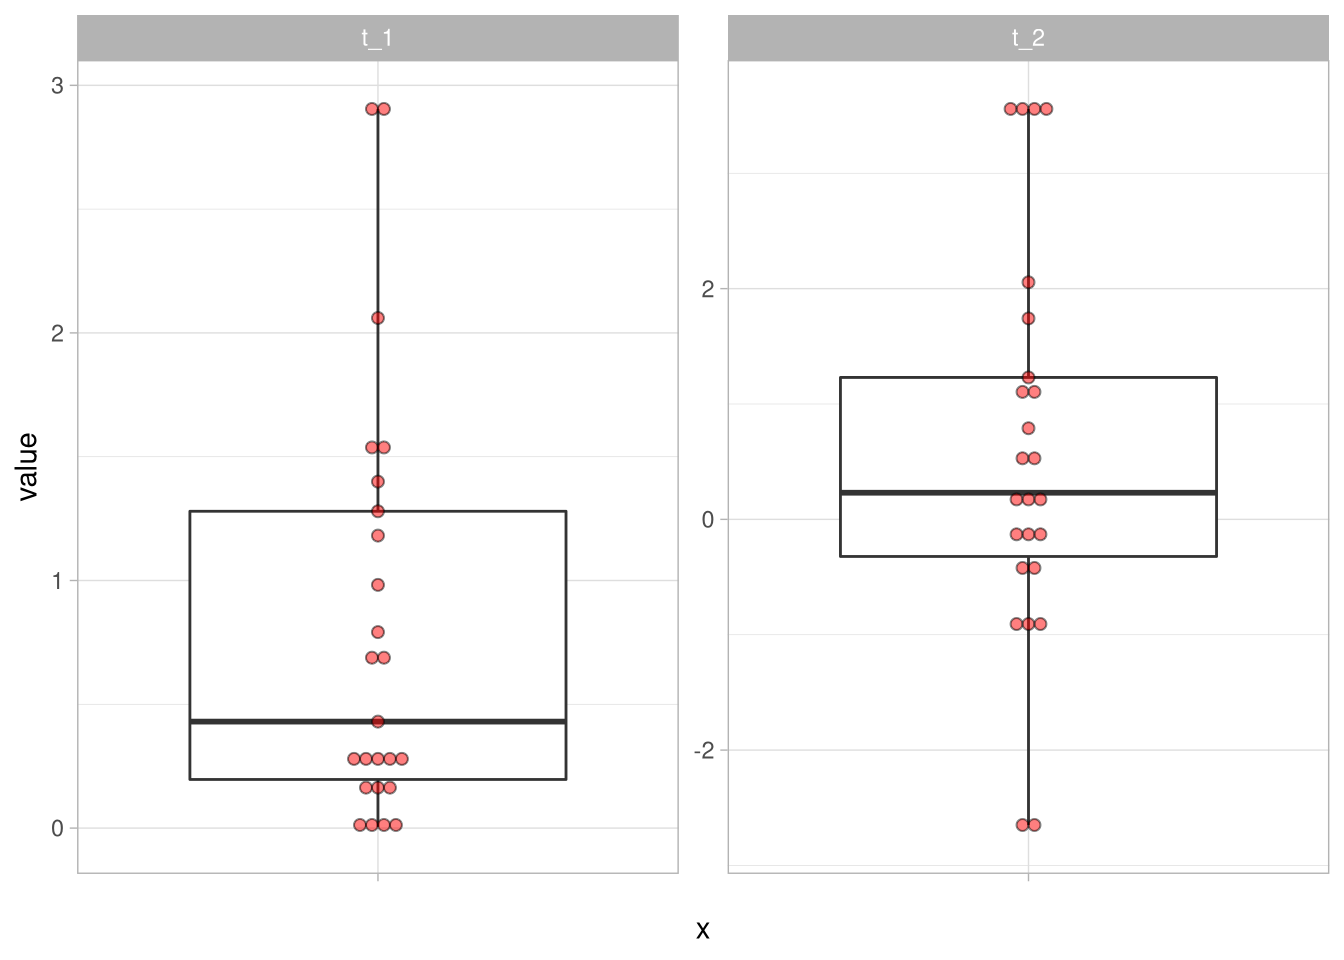
\includegraphics[width=300pt]{EDV2_SS21_files/figure-latex/unnamed-chunk-28-1} \end{center}

\hypertarget{organisationsformen-von-datensuxe4tzen}{%
\section{Organisationsformen von Datensätzen}\label{organisationsformen-von-datensuxe4tzen}}

\hypertarget{long-vs.-wide-format}{%
\subsection{long vs.~wide format}\label{long-vs.-wide-format}}

\begin{cols}

\begin{col}{0.48\textwidth}

\hypertarget{long-format}{%
\paragraph{long-format}\label{long-format}}

\begin{tabular}[t]{lrl}
\toprule
Name & RT & Bedingung\\
\midrule
Snake Müller & 2624 & 1\\
Snake Müller & 3902 & 2\\
Snake Müller & 6293 & 3\\
Vera Baum & 1252 & 1\\
Vera Baum & 2346 & 2\\
\addlinespace
Vera Baum & 4321 & 3\\
\bottomrule
\end{tabular}

\end{col}

\begin{col}{0.48\textwidth}

\hypertarget{wide-format}{%
\paragraph{wide-format}\label{wide-format}}

\begin{tabular}[t]{lrrr}
\toprule
Name & RT\_1 & RT\_2 & RT\_3\\
\midrule
Snake Müller & 2624 & 3902 & 6293\\
Vera Baum & 1252 & 2346 & 4321\\
\bottomrule
\end{tabular}

\end{col}

\end{cols}

Die \texttt{pivot}-Funktionen \texttt{pivot\_longer} und \texttt{pivot\_wider} bieten die Möglichkeit, einen Datensatz von einem in das andere Format zu konvertieren.

\begin{Shaded}
\begin{Highlighting}[]
\NormalTok{longFormat}
\end{Highlighting}
\end{Shaded}

\begin{verbatim}
##           Name   RT Bedingung
## 1 Snake Müller 2624         1
## 2 Snake Müller 3902         2
## 3 Snake Müller 6293         3
## 4    Vera Baum 1252         1
## 5    Vera Baum 2346         2
## 6    Vera Baum 4321         3
\end{verbatim}

\hypertarget{long-to-wide}{%
\subsubsection{long to wide}\label{long-to-wide}}

\begin{Shaded}
\begin{Highlighting}[]
\NormalTok{wideFormat }\OtherTok{\textless{}{-}}\NormalTok{ longFormat }\SpecialCharTok{\%\textgreater{}\%}
  \FunctionTok{pivot\_wider}\NormalTok{(}\AttributeTok{names\_from =} \StringTok{\textquotesingle{}Bedingung\textquotesingle{}}\NormalTok{,}
              \AttributeTok{values\_from =} \StringTok{\textquotesingle{}RT\textquotesingle{}}\NormalTok{,}
              \AttributeTok{names\_prefix =} \StringTok{\textquotesingle{}RT\_\textquotesingle{}}\NormalTok{)}
\NormalTok{wideFormat}
\end{Highlighting}
\end{Shaded}

\begin{verbatim}
## # A tibble: 2 x 4
##   Name          RT_1  RT_2  RT_3
##   <chr>        <dbl> <dbl> <dbl>
## 1 Snake Müller  2624  3902  6293
## 2 Vera Baum     1252  2346  4321
\end{verbatim}

\hypertarget{wide-to-long}{%
\subsubsection{wide to long}\label{wide-to-long}}

\begin{Shaded}
\begin{Highlighting}[]
\NormalTok{longFormat }\OtherTok{\textless{}{-}}\NormalTok{ wideFormat }\SpecialCharTok{\%\textgreater{}\%}
  \FunctionTok{pivot\_longer}\NormalTok{(}\AttributeTok{cols =} \SpecialCharTok{{-}}\DecValTok{1}\NormalTok{,}
               \AttributeTok{names\_prefix =} \StringTok{\textquotesingle{}RT\_\textquotesingle{}}\NormalTok{,}
               \AttributeTok{names\_to =} \StringTok{\textquotesingle{}Bedingung\textquotesingle{}}\NormalTok{,}
               \AttributeTok{values\_to =} \StringTok{\textquotesingle{}RT\textquotesingle{}}\NormalTok{)}
\NormalTok{longFormat}
\end{Highlighting}
\end{Shaded}

\begin{verbatim}
## # A tibble: 6 x 3
##   Name         Bedingung    RT
##   <chr>        <chr>     <dbl>
## 1 Snake Müller 1          2624
## 2 Snake Müller 2          3902
## 3 Snake Müller 3          6293
## 4 Vera Baum    1          1252
## 5 Vera Baum    2          2346
## 6 Vera Baum    3          4321
\end{verbatim}

\hypertarget{hilfsmittel-fuxfcr-die-inferenzstatistik}{%
\chapter{Hilfsmittel für die Inferenzstatistik}\label{hilfsmittel-fuxfcr-die-inferenzstatistik}}

\hypertarget{organisatorisches-1}{%
\section{Organisatorisches}\label{organisatorisches-1}}

\hypertarget{semesterplan-2}{%
\subsection{Semesterplan}\label{semesterplan-2}}

\begin{tabular}[t]{llll}
\toprule
Einheit & Vorlesung & Übungswoche & Thema\\
\midrule
1 & 23.04.21 & keine Übung & Deskriptive Statistik\\
 &  &  & Data Cleaning\\
2 & 07.05.21 & KW 19 & Hilfsmittel für die Inferenzstatistik\\
 &  &  & Lineare Regression I\\
3 & 21.05.21 & KW 21 & Lineare Regression II\\
\addlinespace
4 & 04.06.21 & KW 23 & t- Tests\\
 &  &  & einfaktorielle Varianzanalyse\\
5 & 18.06.21 & KW 25 & zweifaktorielle Varianzanalyse\\
6 & 02.07.21 & KW 27 & Kontrasttests\\
\bottomrule
\end{tabular}

\hypertarget{hilfsmittel-fuxfcr-die-inferenzstatistik-1}{%
\section{Hilfsmittel für die Inferenzstatistik}\label{hilfsmittel-fuxfcr-die-inferenzstatistik-1}}

\hypertarget{modellterme}{%
\subsection{Modellterme}\label{modellterme}}

Alle inferenzstatistischen Verfahren im \texttt{base-R}-Umfang und viele andere aus Zusatzpaketen nutzen die sogenannte \emph{Formelschreibweise} um Modelle zu definieren.
Am Anfang ist die Syntax ein bisschen ungewohnt, am Ende resultiert aus dieser Schreibweise aber eine sehr übersichtliche und schnell erfassbare Modell-Formulierung.

Die Formulierung folgt dabei grundsätzlich dem folgenden System, das sich am Besten analog zu einer mathematischen Funktionsgleichung vorgestellt werden kann. Da das \texttt{=} aber schon für Zuweisungen belegt ist, wird es in \texttt{formula}-Schreibweise durch eine Tilde (\textasciitilde) ersetzt:

 
  \providecommand{\huxb}[2]{\arrayrulecolor[RGB]{#1}\global\arrayrulewidth=#2pt}
  \providecommand{\huxvb}[2]{\color[RGB]{#1}\vrule width #2pt}
  \providecommand{\huxtpad}[1]{\rule{0pt}{#1}}
  \providecommand{\huxbpad}[1]{\rule[-#1]{0pt}{#1}}

\begin{table}[ht]
\begin{centerbox}
\begin{threeparttable}
\captionsetup{justification=centering,singlelinecheck=off}
\caption{\label{tab:unnamed-chunk-39} }
 \setlength{\tabcolsep}{0pt}
\begin{tabular}{l l l l}


\hhline{>{\huxb{255, 255, 255}{0.4}}->{\huxb{0, 0, 0}{0.4}}|>{\huxb{0, 0, 0}{0.4}}->{\huxb{255, 255, 255}{0.4}}->{\huxb{0, 0, 0}{0.4}}|>{\huxb{0, 0, 0}{0.4}}-}
\arrayrulecolor{black}

\multicolumn{1}{!{\huxvb{0, 0, 0}{0}}c!{\huxvb{0, 0, 0}{0.4}}}{\huxtpad{6pt + 1em}\centering \hspace{6pt}  \hspace{6pt}\huxbpad{6pt}} &
\multicolumn{1}{c!{\huxvb{0, 0, 0}{0.4}}}{\huxtpad{6pt + 1em}\centering \hspace{6pt} modellierte Variable(n) \hspace{6pt}\huxbpad{6pt}} &
\multicolumn{1}{c!{\huxvb{0, 0, 0}{0.4}}}{\huxtpad{6pt + 1em}\centering \hspace{6pt} \~{} \hspace{6pt}\huxbpad{6pt}} &
\multicolumn{1}{c!{\huxvb{0, 0, 0}{0.4}}}{\huxtpad{6pt + 1em}\centering \hspace{6pt} Modellformel \hspace{6pt}\huxbpad{6pt}} \tabularnewline[-0.5pt]


\hhline{>{\huxb{255, 255, 255}{0.4}}->{\huxb{0, 0, 0}{0.4}}|>{\huxb{0, 0, 0}{0.4}}->{\huxb{255, 255, 255}{0.4}}->{\huxb{0, 0, 0}{0.4}}|>{\huxb{0, 0, 0}{0.4}}-}
\arrayrulecolor{black}

\multicolumn{1}{!{\huxvb{0, 0, 0}{0}}c!{\huxvb{0, 0, 0}{0}}}{\huxtpad{6pt + 1em}\centering \hspace{6pt}  \hspace{6pt}\huxbpad{6pt}} &
\multicolumn{1}{c!{\huxvb{0, 0, 0}{0}}}{\huxtpad{6pt + 1em}\centering \hspace{6pt}  \hspace{6pt}\huxbpad{6pt}} &
\multicolumn{1}{c!{\huxvb{0, 0, 0}{0}}}{\huxtpad{6pt + 1em}\centering \hspace{6pt}  \hspace{6pt}\huxbpad{6pt}} &
\multicolumn{1}{c!{\huxvb{0, 0, 0}{0}}}{\huxtpad{6pt + 1em}\centering \hspace{6pt}  \hspace{6pt}\huxbpad{6pt}} \tabularnewline[-0.5pt]


\hhline{>{\huxb{255, 255, 255}{0.4}}->{\huxb{0, 0, 0}{0.4}}->{\huxb{255, 255, 255}{0.4}}->{\huxb{0, 0, 0}{0.4}}-}
\arrayrulecolor{black}

\multicolumn{1}{!{\huxvb{0, 0, 0}{0}}c!{\huxvb{0, 0, 0}{0.4}}}{\huxtpad{6pt + 1em}\centering \hspace{6pt} *Regression:* \hspace{6pt}\huxbpad{6pt}} &
\multicolumn{1}{c!{\huxvb{0, 0, 0}{0.4}}}{\huxtpad{6pt + 1em}\centering \hspace{6pt} Kriterium \hspace{6pt}\huxbpad{6pt}} &
\multicolumn{1}{c!{\huxvb{0, 0, 0}{0.4}}}{\huxtpad{6pt + 1em}\centering \hspace{6pt} \~{} \hspace{6pt}\huxbpad{6pt}} &
\multicolumn{1}{c!{\huxvb{0, 0, 0}{0.4}}}{\huxtpad{6pt + 1em}\centering \hspace{6pt} Prädiktor(en) \hspace{6pt}\huxbpad{6pt}} \tabularnewline[-0.5pt]


\hhline{>{\huxb{255, 255, 255}{0.4}}->{\huxb{0, 0, 0}{0.4}}|>{\huxb{0, 0, 0}{0.4}}->{\huxb{255, 255, 255}{0.4}}->{\huxb{0, 0, 0}{0.4}}|>{\huxb{0, 0, 0}{0.4}}-}
\arrayrulecolor{black}

\multicolumn{1}{!{\huxvb{0, 0, 0}{0}}c!{\huxvb{0, 0, 0}{0}}}{\huxtpad{6pt + 1em}\centering \hspace{6pt}  \hspace{6pt}\huxbpad{6pt}} &
\multicolumn{1}{c!{\huxvb{0, 0, 0}{0}}}{\huxtpad{6pt + 1em}\centering \hspace{6pt}  \hspace{6pt}\huxbpad{6pt}} &
\multicolumn{1}{c!{\huxvb{0, 0, 0}{0}}}{\huxtpad{6pt + 1em}\centering \hspace{6pt}  \hspace{6pt}\huxbpad{6pt}} &
\multicolumn{1}{c!{\huxvb{0, 0, 0}{0}}}{\huxtpad{6pt + 1em}\centering \hspace{6pt}  \hspace{6pt}\huxbpad{6pt}} \tabularnewline[-0.5pt]


\hhline{>{\huxb{255, 255, 255}{0.4}}->{\huxb{0, 0, 0}{0.4}}->{\huxb{255, 255, 255}{0.4}}->{\huxb{0, 0, 0}{0.4}}-}
\arrayrulecolor{black}

\multicolumn{1}{!{\huxvb{0, 0, 0}{0}}c!{\huxvb{0, 0, 0}{0.4}}}{\huxtpad{6pt + 1em}\centering \hspace{6pt} *Varianzanalyse:* \hspace{6pt}\huxbpad{6pt}} &
\multicolumn{1}{c!{\huxvb{0, 0, 0}{0.4}}}{\huxtpad{6pt + 1em}\centering \hspace{6pt} AV \hspace{6pt}\huxbpad{6pt}} &
\multicolumn{1}{c!{\huxvb{0, 0, 0}{0.4}}}{\huxtpad{6pt + 1em}\centering \hspace{6pt} \~{} \hspace{6pt}\huxbpad{6pt}} &
\multicolumn{1}{c!{\huxvb{0, 0, 0}{0.4}}}{\huxtpad{6pt + 1em}\centering \hspace{6pt} UV(s als Faktor(en)) \hspace{6pt}\huxbpad{6pt}} \tabularnewline[-0.5pt]


\hhline{>{\huxb{255, 255, 255}{0.4}}->{\huxb{0, 0, 0}{0.4}}|>{\huxb{0, 0, 0}{0.4}}->{\huxb{255, 255, 255}{0.4}}->{\huxb{0, 0, 0}{0.4}}|>{\huxb{0, 0, 0}{0.4}}-}
\arrayrulecolor{black}
\end{tabular}
\end{threeparttable}\par\end{centerbox}

\end{table}
 

\hypertarget{modell-term}{%
\subsubsection{Modell-Term}\label{modell-term}}

Der Modell-Term auf der rechten Seite der Tilde wird dabei aus einer Reihe von Variablen und Kombinationsoperatoren zusammengesetzt. Zuerst etwas unintuitiv sind diese Operatoren im normalen R-Kontext mit anderen Bedeutungen belegt, in \texttt{formula}s funktionieren sie aber so \emph{nicht} Die Operatoren sind die folgenden:

\begin{tabular}[t]{lll}
\toprule
Operator & übliche Bedeutung & Bedeutung in `formula`s\\
\midrule
+ & Addition & Vorhersageterm hinzufügen\\
- & Subtraktion & Vorhersageterm ausschließen\\
<A> : <B> & Sequenz & Interaktion AxB\\
<A> * <B> & Multiplikation & Effekt von A, B und AxB\\
\bottomrule
\end{tabular}

Anhand von einer Reihe von Beispielen wird die Formulierung deutlich, dafür führen wir noch kurz eine Hand voll Notationen ein, die meisten davon sind wahrscheinlich nicht überraschend:

\begin{tabular}[t]{ll}
\toprule
Abkürzung & Bedeutung\\
\midrule
\$H\_0\$ & Nullhypothese eines statistischen Tests\\
\$H\_1\$ & Alternativhypothese eines statistischen Tests\\
\$UV\$ & unabhängige Variable\\
\$AV\$ & abhängige Variable\\
\$X\_i / Y\_i\$ & numerische (Zufalls-) Variable\\
\addlinespace
\$F\_i\$ & kategoriale Varable (Faktor)\\
\bottomrule
\end{tabular}

\hypertarget{regressionsmodelle}{%
\subsubsection{Regressionsmodelle}\label{regressionsmodelle}}

\texttt{Y\ \textasciitilde{}\ X1}: einfache lineare Regression von \texttt{Y} auf \texttt{X1}

\texttt{Y\ \textasciitilde{}\ X1\ +\ X2}: multiple lineare Regression von \texttt{Y} auf \texttt{X1} und \texttt{X2}

\texttt{Y\ \textasciitilde{}\ X1+X2+X1:X2}: multiple lineare Regression von \texttt{Y} auf \texttt{X1} und \texttt{X2} sowie auf den Interaktionsterm von \texttt{X1} und \texttt{X2}

\texttt{Y\ \textasciitilde{}\ X1*X2}: multiple lineare Regression von \texttt{Y} auf \texttt{X1} und \texttt{X2} sowie auf den Interaktionsterm von \texttt{X1} und \texttt{X2}

\hypertarget{varianzanalytische-modelle}{%
\subsubsection{Varianzanalytische Modelle}\label{varianzanalytische-modelle}}

\texttt{Y\ \textasciitilde{}\ F1}: einfaktorielle Varianzanalyse

\texttt{Y\ \textasciitilde{}\ F1\ +\ F2\ +\ F1:F2}: zweifaktorielle Varianzanalyse mit beiden Haupteffekten und der Interaktion

\texttt{Y\ \textasciitilde{}\ F1\ *\ F2}: auch zweifaktorielle Varianzanalyse mit beiden Haupteffekten und der Interaktion

\texttt{Y\ \textasciitilde{}\ X1\ +\ F1}: Kovarianzanalyse mit Kovariate X1 und Faktor F1

Innerhalb einer Modellformel können die Terme selbst das Ergebnis der Anwendung von Funktionen auf Variablen sein:

\[\texttt{log}(Y) \sim \texttt{scale}(X)\]
Wenn wir die für die Formulierung genutzten Operatoren für arithmetische Operationen in der Modellformel verwenden wollen, müssen sie mit \texttt{I()} eingeschlossen werden um den Kontext klarzumachen:

\[Y \sim \texttt{I}(2*X)\]

\hypertarget{aufgabe}{%
\subsection{Aufgabe}\label{aufgabe}}

Welche Hypothese(n) pass(t/en) zu folgender Modellformel:

\begin{Shaded}
\begin{Highlighting}[]
\NormalTok{IQ }\SpecialCharTok{\textasciitilde{}}\NormalTok{ Geschlecht }\SpecialCharTok{+}\NormalTok{ Raucher}
\end{Highlighting}
\end{Shaded}

\begin{itemize}
\item
  A: Es gibt einen Unterschied zwischen der Intelligenz von Rauchern und Nichtrauchern und zwischen der von Frauen und Männern.
\item
  B: Es gibt einen Unterschied zwischen der Intelligenz von Rauchern und Nichtrauchern und zwischen der von Frauen und Männern sowie einen Unterschied in der Intelligenz zwischen Rauchern und Nichtrauchern, der sich in der Ausprägung zwischen den Geschlechtern unterscheidet.
\item
  C: Es gibt einen Unterschied in der Intelligenz zwischen Rauchern und Nichtrauchern, der sich in der Ausprägung zwischen den Geschlechtern unterscheidet.
\item
  D: Es gibt einen Zusammenhang zwischen Rauchen und Geschlecht auf der einen und Intelligenz auf der anderen Seite.
\end{itemize}

Lösung

A ist richtig.

\hypertarget{einfache-lineare-zusammenhuxe4nge}{%
\chapter{Einfache lineare Zusammenhänge}\label{einfache-lineare-zusammenhuxe4nge}}

\hypertarget{datensatz}{%
\subsection{Datensatz}\label{datensatz}}

Für die Tests auf linearen Zusammenhänge werden wir den Datensatz \texttt{df\_wide} mit den folgenden Variablen benutzen:

\begin{tabular}[t]{ll}
\toprule
Variable & Inhalt\\
\midrule
`group` & Treatment-Gruppe\\
`pre\_skill` & motorischer Skill vor dem Treatment\\
`post\_skill` & motorischer Skill nach dem Treatment\\
`hawie\_iq` & Intelligenz-Quotient aus HAWIE\\
`hawie\_wahr\_log` & Skalenwert Wahrnehmungsgebundenes logisches Denken aus HAWIE\\
\bottomrule
\end{tabular}

\hypertarget{test-auf-korrelation}{%
\section{Test auf Korrelation}\label{test-auf-korrelation}}

\hypertarget{test-hintergrund}{%
\subsection{Test-Hintergrund}\label{test-hintergrund}}

Die empirische Korrelation zweier gemeinsam normalverteilter Variablen lässt sich daraufhin testen, ob sie
mit der \(H_0\) `kein linearer Zusammenhang' (\(\text{H}_{0}:\rho_{X,Y} = 0\)) verträglich ist.

Dabei wird genutzt, dass bei Multinormalverteilung und Unkorreliertheit der Variablen \(X\) und \(Y\) die Teststatistik \(t_r = r_{x,y} \sqrt{{n-2}\over{1-r_{x,y}}^2}\) \(t-\)verteilt ist, mit \(n-2\) Freiheitsgraden.

Man testet also die Teststatistik \(t\) gegen die \(t_{n-2}\) -Verteilung.

Ist der Test signifikant, wird die \(H_1\) angenommen, also dass die `wahre' Korrelation zwischen \(X\) und \(Y\) ungleich 0 ist.

Gerichtete Hypothesen lassen sich analog testen.

\hypertarget{test-auf-korrelation-in-r}{%
\subsection{Test auf Korrelation in R}\label{test-auf-korrelation-in-r}}

Man kann den Test in R mit Vektoren als Eingabe\ldots{}

\begin{Shaded}
\begin{Highlighting}[]
\FunctionTok{cor.test}\NormalTok{(df\_wide}\SpecialCharTok{$}\NormalTok{hawie\_iq, df\_wide}\SpecialCharTok{$}\NormalTok{hawie\_wahr\_log)}
\end{Highlighting}
\end{Shaded}

\begin{verbatim}
## 
##  Pearson's product-moment correlation
## 
## data:  df_wide$hawie_iq and df_wide$hawie_wahr_log
## t = 7.0471, df = 48, p-value = 6.228e-09
## alternative hypothesis: true correlation is not equal to 0
## 95 percent confidence interval:
##  0.5424104 0.8272449
## sample estimates:
##       cor 
## 0.7130958
\end{verbatim}

\ldots{} und mit Modellformel als Eingabe aufrufen.

\begin{Shaded}
\begin{Highlighting}[]
\FunctionTok{cor.test}\NormalTok{(}\SpecialCharTok{\textasciitilde{}}\NormalTok{ hawie\_iq }\SpecialCharTok{+}\NormalTok{ hawie\_wahr\_log, }\AttributeTok{data =}\NormalTok{ df\_wide)}
\end{Highlighting}
\end{Shaded}

\begin{verbatim}
## 
##  Pearson's product-moment correlation
## 
## data:  hawie_iq and hawie_wahr_log
## t = 7.0471, df = 48, p-value = 6.228e-09
## alternative hypothesis: true correlation is not equal to 0
## 95 percent confidence interval:
##  0.5424104 0.8272449
## sample estimates:
##       cor 
## 0.7130958
\end{verbatim}

Das \texttt{alternative}-Argument bietet die Möglichkeit, die Richtung des Signifikanztests anzugeben.

Dabei steht \texttt{\textquotesingle{}greater\textquotesingle{}} für einen rechtsseitigen, \texttt{\textquotesingle{}lesser\textquotesingle{}} für einen linksseitigen und der Standard \texttt{\textquotesingle{}two.sided\textquotesingle{}} für einen zweiseitigen Test.

\begin{Shaded}
\begin{Highlighting}[]
\FunctionTok{cor.test}\NormalTok{(}\SpecialCharTok{\textasciitilde{}}\NormalTok{ hawie\_iq }\SpecialCharTok{+}\NormalTok{ hawie\_wahr\_log, }
         \AttributeTok{data =}\NormalTok{ df\_wide,}
         \AttributeTok{alternative=}\StringTok{\textquotesingle{}greater\textquotesingle{}}\NormalTok{) }
\end{Highlighting}
\end{Shaded}

\begin{verbatim}
## 
##  Pearson's product-moment correlation
## 
## data:  hawie_iq and hawie_wahr_log
## t = 7.0471, df = 48, p-value = 3.114e-09
## alternative hypothesis: true correlation is greater than 0
## 95 percent confidence interval:
##  0.5740402 1.0000000
## sample estimates:
##       cor 
## 0.7130958
\end{verbatim}

Der Output lässt sich noch ein bisschen schicker mit der \texttt{tidy}-Funktion aus dem \texttt{broom}-Paket darstellen (ist auch im \texttt{tidyverse} enthalten):

\begin{Shaded}
\begin{Highlighting}[]
\FunctionTok{cor.test}\NormalTok{(}\SpecialCharTok{\textasciitilde{}}\NormalTok{ hawie\_iq }\SpecialCharTok{+}\NormalTok{ hawie\_wahr\_log, }
         \AttributeTok{data =}\NormalTok{ df\_wide,}
         \AttributeTok{alternative=}\StringTok{\textquotesingle{}greater\textquotesingle{}}\NormalTok{) }\SpecialCharTok{\%\textgreater{}\%} 
\NormalTok{  broom}\SpecialCharTok{::}\FunctionTok{tidy}\NormalTok{()}
\end{Highlighting}
\end{Shaded}

\begin{verbatim}
## # A tibble: 1 x 8
##   estimate statistic       p.value parameter conf.low
##      <dbl>     <dbl>         <dbl>     <int>    <dbl>
## 1    0.713      7.05 0.00000000311        48    0.574
##   conf.high method                              
##       <dbl> <chr>                               
## 1         1 Pearson's product-moment correlation
##   alternative
##   <chr>      
## 1 greater
\end{verbatim}

\hypertarget{aufgabe-1}{%
\subsection{Aufgabe}\label{aufgabe-1}}

Wie kann ich das Ergebnis interpretieren?

\begin{Shaded}
\begin{Highlighting}[]
\FunctionTok{cor.test}\NormalTok{(}\SpecialCharTok{\textasciitilde{}}\NormalTok{ hawie\_iq }\SpecialCharTok{+}\NormalTok{ hawie\_wahr\_log, }
         \AttributeTok{data =}\NormalTok{ df\_wide,}
         \AttributeTok{alternative=}\StringTok{\textquotesingle{}greater\textquotesingle{}}\NormalTok{) }\SpecialCharTok{\%\textgreater{}\%} 
\NormalTok{  broom}\SpecialCharTok{::}\FunctionTok{tidy}\NormalTok{()}
\end{Highlighting}
\end{Shaded}

\begin{verbatim}
## # A tibble: 1 x 8
##   estimate statistic       p.value parameter conf.low
##      <dbl>     <dbl>         <dbl>     <int>    <dbl>
## 1    0.713      7.05 0.00000000311        48    0.574
##   conf.high method                              
##       <dbl> <chr>                               
## 1         1 Pearson's product-moment correlation
##   alternative
##   <chr>      
## 1 greater
\end{verbatim}

\begin{itemize}
\tightlist
\item
  A: Die Logik-Leitung beeinflusst den IQ signifikant positiv.
\item
  B: Es gibt keine Korrelation zwischen Logik-Leistung und IQ.
\item
  C: Die Logik-Leistung und der IQ sind signifikant von Null unterschiedlich korreliert.
\item
  D: Es gibt einen signifikanten, positiv linearen Zusammenhang zwischen Logik-Leistung und IQ.
\end{itemize}

Lösung

C und D könnte man so sagen, D hat aber natürlich mehr Informationsgehalt.

\hypertarget{einfache-lineare-regression}{%
\section{Einfache lineare Regression}\label{einfache-lineare-regression}}

\hypertarget{modellanpassung}{%
\subsection{Modellanpassung}\label{modellanpassung}}

Bei der einfachen linearen Regression werden anhand der paarweise vorhandenen Daten zweier
Variablen X und Y die Parameter a und b der Vorhersagegleichung \(\hat{Y} = bX + a\) so bestimmt,
dass die Werte von \(Y\) (dem Kriterium) bestmöglich mit der Vorhersage \(\hat{Y}\) aus den Werten
von \(X\) (dem Prädiktor) übereinstimmen.

Als Maß für die Güte der Vorhersage wird die
Summe der quadrierten Residuen \(E = Y - \hat{Y}\) , also der Abweichungen von vorhergesagten und
Kriteriumswerten herangezogen.

Lineare Modelle wie das der Regression lassen sich mit lm() anpassen und so die Parameter a und b schätzen.

\begin{Shaded}
\begin{Highlighting}[]
\FunctionTok{lm}\NormalTok{(}\AttributeTok{formula=} \SpecialCharTok{\textless{}}\NormalTok{Modellformel}\SpecialCharTok{\textgreater{}}\NormalTok{ , }\AttributeTok{data=}\SpecialCharTok{\textless{}}\NormalTok{Datensatz}\SpecialCharTok{\textgreater{}}\NormalTok{)}
\end{Highlighting}
\end{Shaded}

Ein von lm() zurückgegebenes Objekt stellt ein deskriptives Modell der Daten dar, das in anderen Funktionen weiter verwendet werden kann.

\hypertarget{beispiel-fuxfcr-deskriptive-modellanpassung}{%
\subsubsection{Beispiel für deskriptive Modellanpassung}\label{beispiel-fuxfcr-deskriptive-modellanpassung}}

Als Beispiel soll die Leistung auf der Skala zum wahrnehmungsgebundenen logischen Denken als Kriterium mit dem IQ als Prädiktor vorhergesagt werden.

\begin{Shaded}
\begin{Highlighting}[]
\NormalTok{(fitI }\OtherTok{\textless{}{-}} \FunctionTok{lm}\NormalTok{(hawie\_wahr\_log }\SpecialCharTok{\textasciitilde{}}\NormalTok{ hawie\_iq, }\AttributeTok{data =}\NormalTok{ df\_wide)) }
\end{Highlighting}
\end{Shaded}

\begin{verbatim}
## 
## Call:
## lm(formula = hawie_wahr_log ~ hawie_iq, data = df_wide)
## 
## Coefficients:
## (Intercept)     hawie_iq  
##     -3.2874       0.1301
\end{verbatim}

\begin{Shaded}
\begin{Highlighting}[]
\FunctionTok{ggplot}\NormalTok{(df\_wide, }\FunctionTok{aes}\NormalTok{(}\AttributeTok{x =}\NormalTok{ hawie\_iq, }\AttributeTok{y =}\NormalTok{ hawie\_wahr\_log)) }\SpecialCharTok{+}
  \FunctionTok{geom\_point}\NormalTok{() }\SpecialCharTok{+}
  \FunctionTok{geom\_smooth}\NormalTok{(}\AttributeTok{formula =}\NormalTok{  y }\SpecialCharTok{\textasciitilde{}}\NormalTok{ x ,}
              \AttributeTok{method =} \StringTok{\textquotesingle{}lm\textquotesingle{}}\NormalTok{,}\AttributeTok{col =}\StringTok{\textquotesingle{}red\textquotesingle{}}\NormalTok{,}\AttributeTok{se =}\NormalTok{ F)}
\end{Highlighting}
\end{Shaded}

\begin{center}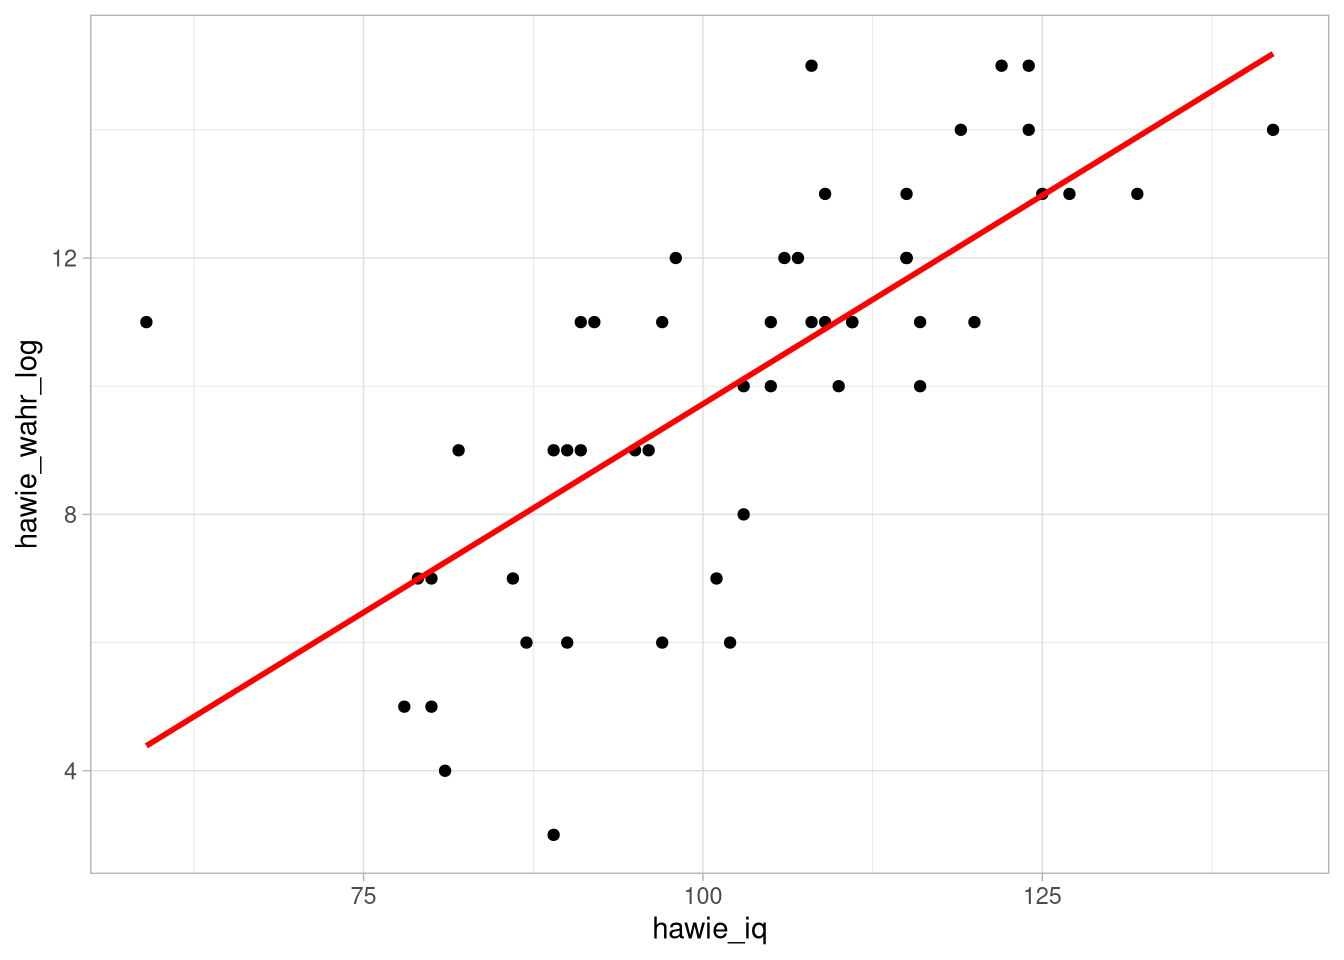
\includegraphics[width=166.666666666667pt]{EDV2_SS21_files/figure-latex/unnamed-chunk-52-1} \end{center}

\hypertarget{beta-gewicht}{%
\subsection{\texorpdfstring{\(\beta\)-Gewicht}{\textbackslash beta-Gewicht}}\label{beta-gewicht}}

Will man statt des \(b\)-Gewichtes das standardisierte \(\beta\)-Gewicht angeben, muss in der Modellformel z-transformiert werden.

Dafür könenn wir entweder alle Teile der \texttt{formula} \texttt{scale}n:

\begin{Shaded}
\begin{Highlighting}[]
\NormalTok{(fitZ }\OtherTok{\textless{}{-}} \FunctionTok{lm}\NormalTok{(}\FunctionTok{scale}\NormalTok{(hawie\_wahr\_log) }\SpecialCharTok{\textasciitilde{}} \FunctionTok{scale}\NormalTok{(hawie\_iq), }
            \AttributeTok{data =}\NormalTok{ df\_wide))}
\end{Highlighting}
\end{Shaded}

\begin{verbatim}
## 
## Call:
## lm(formula = scale(hawie_wahr_log) ~ scale(hawie_iq), data = df_wide)
## 
## Coefficients:
##     (Intercept)  scale(hawie_iq)  
##      -2.284e-16        7.131e-01
\end{verbatim}

Oder wir benutzen die Index-pipe \texttt{\%\$\%} aus dem \texttt{magrittr}-Paket und ein zwischengeschaltetes \texttt{mutate}, um die Skalierung ein bisschen übersichtlicher zu gestalten:

\begin{Shaded}
\begin{Highlighting}[]
\FunctionTok{library}\NormalTok{(magrittr)}
\NormalTok{fitZ }\OtherTok{\textless{}{-}}\NormalTok{ df\_wide }\SpecialCharTok{\%\textgreater{}\%} 
  \FunctionTok{mutate}\NormalTok{(}\AttributeTok{hawie\_wahr\_log =} \FunctionTok{scale}\NormalTok{(hawie\_wahr\_log),}
         \AttributeTok{hawie\_iq =} \FunctionTok{scale}\NormalTok{(hawie\_iq)) }\SpecialCharTok{\%$\%}
  \FunctionTok{lm}\NormalTok{(hawie\_wahr\_log }\SpecialCharTok{\textasciitilde{}}\NormalTok{ hawie\_iq)}

\NormalTok{fitZ}
\end{Highlighting}
\end{Shaded}

\begin{verbatim}
## 
## Call:
## lm(formula = hawie_wahr_log ~ hawie_iq)
## 
## Coefficients:
## (Intercept)     hawie_iq  
##  -2.284e-16    7.131e-01
\end{verbatim}

\begin{Shaded}
\begin{Highlighting}[]
\NormalTok{df\_wide }\SpecialCharTok{\%\textgreater{}\%} 
  \FunctionTok{mutate}\NormalTok{(}\AttributeTok{hawie\_wahr\_log =} \FunctionTok{scale}\NormalTok{(hawie\_wahr\_log),}
         \AttributeTok{hawie\_iq =} \FunctionTok{scale}\NormalTok{(hawie\_iq)) }\SpecialCharTok{\%\textgreater{}\%} 
  \FunctionTok{ggplot}\NormalTok{(}\FunctionTok{aes}\NormalTok{(}\AttributeTok{x =} \FunctionTok{scale}\NormalTok{(hawie\_iq), }
                      \AttributeTok{y =} \FunctionTok{scale}\NormalTok{(hawie\_wahr\_log))) }\SpecialCharTok{+}
    \FunctionTok{geom\_point}\NormalTok{() }\SpecialCharTok{+}
    \FunctionTok{geom\_smooth}\NormalTok{(}\AttributeTok{formula =}\NormalTok{  y }\SpecialCharTok{\textasciitilde{}}\NormalTok{ x ,}
                \AttributeTok{method =} \StringTok{\textquotesingle{}lm\textquotesingle{}}\NormalTok{,}\AttributeTok{col =}\StringTok{\textquotesingle{}red\textquotesingle{}}\NormalTok{,}\AttributeTok{se =}\NormalTok{ F)}
\end{Highlighting}
\end{Shaded}

\begin{center}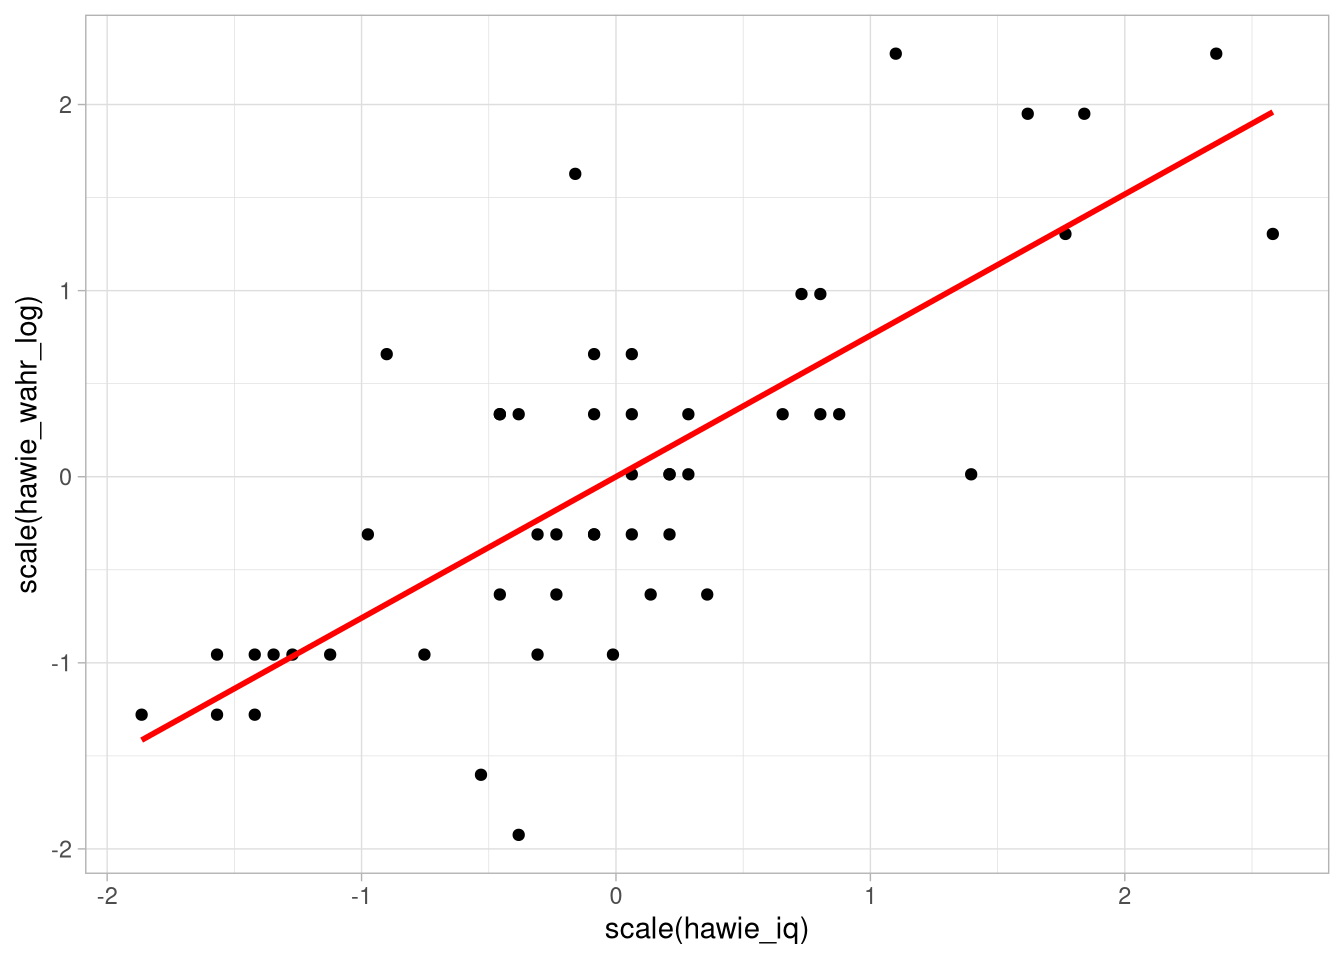
\includegraphics[width=166.666666666667pt]{EDV2_SS21_files/figure-latex/unnamed-chunk-55-1} \end{center}

\hypertarget{weitere-parameter}{%
\subsection{weitere Parameter}\label{weitere-parameter}}

\texttt{lm()} gibt eine Liste zurück, die ein deskriptives Modell der Daten darstellt.

R bietet weitere Funktionen um einzelne Parameter dieses Outputs auszulesen.

Zum Beispiel:
\texttt{residuals()} zum Anzeigen der Residuen, \texttt{coef()} zur Ausgabe der geschätzten Modellparameter und \texttt{fitted()} für die vorhergesagten Werte.

\begin{Shaded}
\begin{Highlighting}[]
\FunctionTok{residuals}\NormalTok{(fitZ)}
\end{Highlighting}
\end{Shaded}

\begin{verbatim}
##            1            2            3            4 
## -0.051410121 -0.124304792  2.196986725  0.843014168 
##            5            6            7            8 
## -0.394825317  0.107961353  0.235184545 -1.080533632 
##            9           10           11           12 
##  0.537853351 -0.675313884 -0.704970155  0.813357897 
##           13           14           15           16 
##  0.002918400  0.440286430  0.715790976  0.191946144 
##           17           18           19           20 
##  0.107961353 -0.051410121 -0.040320001  0.035066681 
##           21           22           23           24 
## -1.107697893 -0.267602125  0.007902421 -0.440555728 
##           25           26           27           28 
## -1.758765916 -0.024245860 -0.702478144  0.453868560 
##           29           30           31           32 
##  0.383465899  0.553927492 -0.037827990  0.208020285 
##           33           34           35           36 
## -0.340496797 -0.067484261  0.770119496 -0.294766385 
##           37           38           39           40 
##  0.148707743  0.699716835  0.497106961  1.407605390 
##           41           42           43           44 
##  0.599657903  0.802267777 -0.299750406  0.078305082 
##           45           46           47           48 
## -0.948326419 -0.618493353 -0.805029086 -1.323889897 
##           49           50 
## -0.078574381 -0.599927202 
## attr(,"scaled:center")
## [1] 10.08
## attr(,"scaled:scale")
## [1] 3.009102
\end{verbatim}

Im \texttt{broom}-Paket gibt es außerdem die \texttt{augment}-Funktion, die uns den zum Fitten genutzten Datensatz mit einer Reihe von Zusatzinfos ausgibt.

\begin{Shaded}
\begin{Highlighting}[]
\NormalTok{broom}\SpecialCharTok{::}\FunctionTok{augment}\NormalTok{(fitZ)}
\end{Highlighting}
\end{Shaded}

\begin{verbatim}
## # A tibble: 50 x 8
##    hawie_wahr_log[,1] hawie_iq[,1] .fitted  .resid
##                 <dbl>        <dbl>   <dbl>   <dbl>
##  1             0.306         0.501  0.357  -0.0514
##  2            -0.0266        0.137  0.0977 -0.124 
##  3             0.306        -2.65  -1.89    2.20  
##  4             0.638        -0.287 -0.205   0.843 
##  5             1.30          2.38   1.70   -0.395 
##  6             0.638         0.743  0.530   0.108 
##  7            -0.359        -0.833 -0.594   0.235 
##  8            -2.02         -1.32  -0.940  -1.08  
##  9            -0.359        -1.26  -0.897   0.538 
## 10            -1.36         -0.954 -0.681  -0.675 
##      .hat .sigma   .cooksd .std.resid
##     <dbl>  <dbl>     <dbl>      <dbl>
##  1 0.0251  0.716 0.0000696    -0.0735
##  2 0.0204  0.716 0.000327     -0.177 
##  3 0.164   0.624 1.12          3.39  
##  4 0.0217  0.705 0.0160        1.20  
##  5 0.136   0.713 0.0282       -0.600 
##  6 0.0313  0.716 0.000387      0.155 
##  7 0.0342  0.715 0.00202       0.338 
##  8 0.0555  0.697 0.0723       -1.57  
##  9 0.0523  0.711 0.0168        0.780 
## 10 0.0386  0.709 0.0190       -0.972 
## # ... with 40 more rows
\end{verbatim}

\begin{Shaded}
\begin{Highlighting}[]
\NormalTok{fitZ }\SpecialCharTok{\%\textgreater{}\%} 
\NormalTok{  broom}\SpecialCharTok{::}\FunctionTok{augment}\NormalTok{() }\SpecialCharTok{\%\textgreater{}\%} 
  \FunctionTok{ggplot}\NormalTok{(}\FunctionTok{aes}\NormalTok{(}\AttributeTok{x =}\NormalTok{ hawie\_iq, }
             \AttributeTok{y =}\NormalTok{ hawie\_wahr\_log))}\SpecialCharTok{+}
  \FunctionTok{geom\_linerange}\NormalTok{(}\FunctionTok{aes}\NormalTok{(}\AttributeTok{ymin =}\NormalTok{ .fitted, }\AttributeTok{ymax =}\NormalTok{ hawie\_wahr\_log), }\AttributeTok{col =} \StringTok{\textquotesingle{}orange\textquotesingle{}}\NormalTok{) }\SpecialCharTok{+}
    \FunctionTok{geom\_point}\NormalTok{() }\SpecialCharTok{+}
    \FunctionTok{geom\_smooth}\NormalTok{(}\AttributeTok{formula =}\NormalTok{  y }\SpecialCharTok{\textasciitilde{}}\NormalTok{ x ,}
                \AttributeTok{method =} \StringTok{\textquotesingle{}lm\textquotesingle{}}\NormalTok{,}\AttributeTok{col =}\StringTok{\textquotesingle{}red\textquotesingle{}}\NormalTok{,}\AttributeTok{se =}\NormalTok{ F)}
\end{Highlighting}
\end{Shaded}

\begin{center}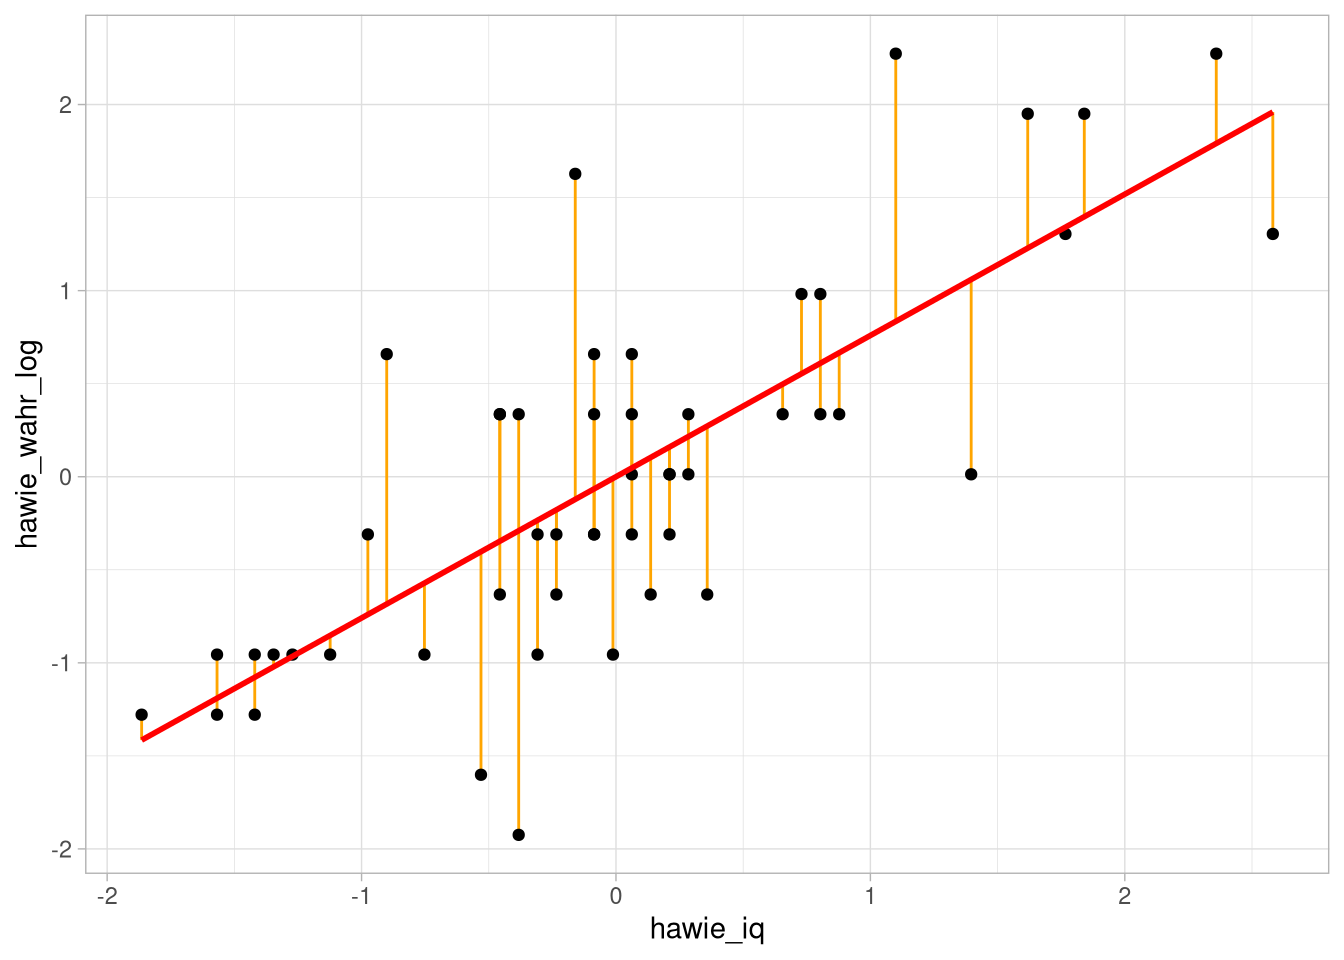
\includegraphics[width=166.666666666667pt]{EDV2_SS21_files/figure-latex/unnamed-chunk-58-1} \end{center}

\hypertarget{regressionsanalyse}{%
\section{Regressionsanalyse}\label{regressionsanalyse}}

\hypertarget{test-hintergrund-1}{%
\subsection{Test-Hintergrund}\label{test-hintergrund-1}}

Unter Voraussetzungen von Varianzhomogenität und Normalverteilung der \(Y\)-Werte für jeden möglichen Wert von \(X\) können Regressionskoeffizienten ähnlich wie Korrelationskoeffizienten auf Unterschiedlichkeit von 0 getestet werden.

Dazu wird genutzt, dass der Term \(t = {{b}\over{{s_{Y \cdot X}}\over {s_X \sqrt{N-1}}}}\) \(t_{N-1}\)-verteilt ist, wenn das tatsächliche \(b^*\) nicht unterschiedlich von 0 ist und für jeden Wert von \(X\) \(Y\) normalverteilt ist mit \(\mu = b^*X + a^*\) und einer Varianz \(\sigma^2\). Die Nullhypothese ist also \(\text{H}_0: b^* = 0\).

\hypertarget{test-in-r}{%
\subsection{Test in R}\label{test-in-r}}

Um zusätzliche Informationen (insbesondere inferenzstatistische Kennwerte) eine mit \texttt{lm()} erstellten Regressions-Modells zu erhalten, kann einfach \texttt{summary()} verwendet werden.

\begin{Shaded}
\begin{Highlighting}[]
\NormalTok{fitZ }\SpecialCharTok{\%\textgreater{}\%} 
  \FunctionTok{summary}\NormalTok{()}
\end{Highlighting}
\end{Shaded}

\begin{verbatim}
## 
## Call:
## lm(formula = hawie_wahr_log ~ hawie_iq)
## 
## Residuals:
##      Min       1Q   Median       3Q      Max 
## -1.75877 -0.38124 -0.01066  0.45047  2.19699 
## 
## Coefficients:
##               Estimate Std. Error t value Pr(>|t|)
## (Intercept) -2.284e-16  1.002e-01   0.000        1
## hawie_iq     7.131e-01  1.012e-01   7.047 6.23e-09
##                
## (Intercept)    
## hawie_iq    ***
## ---
## Signif. codes:  
## 0 '***' 0.001 '**' 0.01 '*' 0.05 '.' 0.1 ' ' 1
## 
## Residual standard error: 0.7083 on 48 degrees of freedom
## Multiple R-squared:  0.5085, Adjusted R-squared:  0.4983 
## F-statistic: 49.66 on 1 and 48 DF,  p-value: 6.228e-09
\end{verbatim}

Außerdem gibt es auch hier einen hübschen \texttt{broom}-Output, für den wir mit \texttt{conf.int} angeben können, Konfidenzintervalle für die Regressionsgewichte ausgeben lassen zu wollen:

\begin{Shaded}
\begin{Highlighting}[]
\NormalTok{fitZ }\SpecialCharTok{\%\textgreater{}\%} 
\NormalTok{  broom}\SpecialCharTok{::}\FunctionTok{tidy}\NormalTok{(}\AttributeTok{conf.int =}\NormalTok{ T)}
\end{Highlighting}
\end{Shaded}

\begin{verbatim}
## # A tibble: 2 x 7
##   term         estimate std.error statistic
##   <chr>           <dbl>     <dbl>     <dbl>
## 1 (Intercept) -2.28e-16     0.100 -2.28e-15
## 2 hawie_iq     7.13e- 1     0.101  7.05e+ 0
##         p.value conf.low conf.high
##           <dbl>    <dbl>     <dbl>
## 1 1.00            -0.201     0.201
## 2 0.00000000623    0.510     0.917
\end{verbatim}

\hypertarget{aufgabe-2}{%
\subsection{Aufgabe}\label{aufgabe-2}}

\begin{Shaded}
\begin{Highlighting}[]
\NormalTok{fitZ }\SpecialCharTok{\%\textgreater{}\%} 
\NormalTok{  broom}\SpecialCharTok{::}\FunctionTok{tidy}\NormalTok{(}\AttributeTok{conf.int =}\NormalTok{ T)}
\end{Highlighting}
\end{Shaded}

\begin{verbatim}
## # A tibble: 2 x 7
##   term         estimate std.error statistic
##   <chr>           <dbl>     <dbl>     <dbl>
## 1 (Intercept) -2.28e-16     0.100 -2.28e-15
## 2 hawie_iq     7.13e- 1     0.101  7.05e+ 0
##         p.value conf.low conf.high
##           <dbl>    <dbl>     <dbl>
## 1 1.00            -0.201     0.201
## 2 0.00000000623    0.510     0.917
\end{verbatim}

\textbf{Wie lässt sich das Ergebnis interpretieren?}
* A: Höhere IQ-Werte hängen mit höheren Logik-Leistungswerten zusammen.
* B: Es gibt keine Korrelation zwischen IQ-Werten und Logik-Leistung.
* C: Mit jedem Anstieg des IQ um eine Streuungs-Einheit, steigt die Vorhersage um 0.7130958 Streuungs-Einheiten.
* D: Man kann wegen der unzureichenden Berücksichtigung nicht-linearer Zusammenhänge keine Aussage treffen.

Lösung

C könnte man so sagen.

  \bibliography{book.bib,packages.bib}

\end{document}
